\chapter{Metodología y Desarrollo del Producto}\label{desarrollo-del-producto}

Este capítulo recorre el trabajo realizado: primero cómo se organizó con el cliente, después el problema y los requerimientos del sistema, luego el tratamiento de los datos, la experimentación y el modelo de línea base, y por último la gestión de riesgos e impacto del producto.

\section{Metodología de trabajo aplicada}\label{sec:metodologia-aplicada}

Esta sección describe cómo se organizó el trabajo con el cliente y entre los autores, siguiendo el enfoque híbrido presentado en la \cref{sec:metodologias-agiles}. El proyecto se inició en la segunda semana de febrero de 2026 y atravesó dos etapas con lógicas de gestión distintas: una etapa de descubrimiento, conducida con iteraciones semanales al estilo de Scrum, y una etapa de ejecución, gestionada con un tablero Kanban.

\subsection{Roles y partes del equipo}\label{ssec:roles}

El equipo de trabajo quedó integrado por tres partes. Por el Ministerio Público Fiscal participó un representante de la Unidad Judicial de Accidentología Vial, que actuó como referente funcional: conocía el proceso, los recursos y las decisiones que el sistema debía apoyar. Por LIDeSIA participó su directora, tutora de este trabajo, que aportó la dirección técnica y el vínculo institucional del convenio. Los autores asumieron el desarrollo y, de manera compartida, la priorización del trabajo, una función análoga a la del \eng{Product Owner} de Scrum. No se designó un \eng{Scrum Master} formal; la facilitación de las reuniones quedó a cargo de los propios autores.

\subsection{Etapa de descubrimiento: iteraciones semanales con el cliente}\label{ssec:descubrimiento}

Entre la segunda semana de febrero y fines de marzo de 2026 se trabajó en iteraciones de una semana. Cada iteración cerraba con una reunión de revisión entre los autores, el representante de la Unidad Judicial y la directora de LIDeSIA, en la que se presentaba lo avanzado, se discutían las dudas sobre el proceso judicial y se acordaban los temas de la semana siguiente. Estas reuniones cumplieron a la vez el rol de revisión del \eng{sprint} y de principal instrumento de relevamiento de requerimientos (\cref{sec:objeto-requerimientos}). La \cref{tab:iteraciones} agrupa las iteraciones por el tema que predominó en ellas.

% VERIFICAR: la cronología de la tabla es una reconstrucción por temas; confirmar los períodos.
{\setstretch{1.0}\small
\begin{longtable}{@{}>{\raggedright\arraybackslash}p{0.15\textwidth}
                    >{\raggedright\arraybackslash}p{0.22\textwidth}
                    >{\raggedright\arraybackslash}p{0.33\textwidth}
                    >{\raggedright\arraybackslash}p{0.22\textwidth}@{}}
\caption{Iteraciones de la etapa de descubrimiento}
\label{tab:iteraciones} \\
\toprule
\textbf{Período} & \textbf{Pregunta de trabajo} & \textbf{Resultado} & \textbf{Producto} \\
\midrule
\endfirsthead
\multicolumn{4}{@{}l}{\footnotesize\textit{Tabla \ref{tab:iteraciones} (continuación)}} \\
\toprule
\textbf{Período} & \textbf{Pregunta de trabajo} & \textbf{Resultado} & \textbf{Producto} \\
\midrule
\endhead
\bottomrule
\endfoot
Febrero, semanas 2 y 3 & ¿Cómo es el proceso ante un siniestro y qué recursos moviliza? & Comprensión del circuito entre la Unidad Judicial, Policía Judicial y los gabinetes periciales. & Diagrama del procedimiento judicial (\cref{fig:procedimiento-judicial-siniestro}). \\
Febrero, semana 4, y marzo, semana 1 & ¿Quién usaría el sistema y qué decisión debería apoyar? & Identificación de usuarios, de no usuarios y de partes interesadas; la planificación de recursos como decisión objetivo. & Necesidad y partes interesadas (\cref{sec:necesidad,sec:objeto-requerimientos}). \\
Marzo, semanas 2 y 3 & ¿Qué datos existen y cuándo están disponibles? & Conocimiento de la base, de su latencia de carga y de su granularidad; adopción del bloque de seis horas a partir de la experiencia del personal del MPF. & Unidad de agregación y restricciones de datos. \\
Marzo, semana 4 & ¿Cómo debe comunicarse el riesgo? & Preferencia por una escala de colores simple y por un sistema explicable, de código abierto y alojado en el CCAD. & Especificación de la capa de decisión y requerimientos no funcionales. \\
\end{longtable}
}
\notaflot{\fuentepropia. Cada período agrupa una o dos iteraciones semanales cerradas con reunión de revisión.}

\subsection{Etapa de ejecución: tablero Kanban}\label{ssec:ejecucion}

Hacia fines de marzo las necesidades del organismo estaban lo suficientemente claras como para planificar el resto del proyecto. A partir de ese momento el trabajo dejó de depender de la revisión semanal con el cliente y pasó a ser, en su mayor parte, una corriente de tareas técnicas (limpieza de datos, ingeniería de variables, entrenamiento de modelos, redacción) cuya prioridad cambiaba según los resultados que se iban obteniendo. Por ese motivo los autores organizaron su trabajo en un tablero Kanban con cuatro columnas: pendiente, en curso, en revisión y terminado. La columna de revisión correspondía a las entregas parciales que se sometían a la tutora antes de darlas por cerradas. Las fases del cronograma de la \cref{fig:gantt-proyecto} funcionaron como horizonte de planificación, y el tablero, como herramienta para decidir qué hacer cada semana dentro de ellas.

\subsection{Cambios durante el proyecto}\label{ssec:cambios}

El proyecto sufrió numerosos cambios de rumbo, y la capacidad de absorberlos sin perder el objetivo fue una de las principales pruebas que debió superar. La \cref{tab:cambios-proyecto} reúne los más relevantes, su causa y la respuesta adoptada.

{\setstretch{1.0}\small
\begin{longtable}{@{}>{\raggedright\arraybackslash}p{0.30\textwidth}
                    >{\raggedright\arraybackslash}p{0.30\textwidth}
                    >{\raggedright\arraybackslash}p{0.34\textwidth}@{}}
\caption{Principales cambios durante el proyecto}
\label{tab:cambios-proyecto} \\
\toprule
\textbf{Cambio} & \textbf{Causa} & \textbf{Respuesta} \\
\midrule
\endfirsthead
\multicolumn{3}{@{}l}{\footnotesize\textit{Tabla \ref{tab:cambios-proyecto} (continuación)}} \\
\toprule
\textbf{Cambio} & \textbf{Causa} & \textbf{Respuesta} \\
\midrule
\endhead
\bottomrule
\endfoot
Variable objetivo: de la cantidad de víctimas a la presencia de al menos una víctima por bloque. & Los modelos de conteo y de tres clases no alcanzaban un desempeño útil (\cref{ap:experimentos}). & Variable binaria \var{TARGET\_CRITICO} con un regresor de Poisson y una capa de decisión. \\
Enfoque de modelado: de modelos fundacionales y redes neuronales a árboles de decisión. & Volumen de datos acotado y exigencia de explicabilidad. & Selección de XGBoost como modelo de línea base (\cref{pipeline-del-modelo-de-luxednea-base-baseline}). \\
Predicción por zonas de la ciudad. & Baja densidad de siniestros por celda y riesgo de uso desviado. & Se exploró de forma experimental y se dejó fuera del alcance (\cref{sec:alcance}). \\
Versiones sucesivas de la base de datos y datos climáticos poco confiables. & Revisiones del equipo de datos del MPF. & Reprocesamiento de la base y obtención del clima desde una fuente externa. \\
Variables con fuga de información. & Campos administrativos que se completan después del hecho. & Detección y descarte antes del entrenamiento (\cref{exploraciuxf3n-de-datos}). \\
Límites de cómputo en el CCAD. & Trabajos interrumpidos por el tiempo máximo de ejecución de los clústeres. & Rediseño de los entrenamientos en corridas más cortas y reproducibles. \\
\end{longtable}
}
\notaflot{\fuentepropia.}

Ninguno de estos cambios estaba previsto en la planificación inicial. El tablero Kanban permitió incorporarlos sin rehacer el plan: cada cambio se traducía en tareas nuevas que entraban a la columna de pendientes y se priorizaban frente a las existentes. El costo de esa flexibilidad fue que las tareas de experimentación con modelos, más urgentes en el día a día, tendieron a desplazar a las de gestión del producto.

\subsection{Balance de la metodología}\label{ssec:balance-metodologia}

La etapa de descubrimiento cumplió su propósito. Las revisiones semanales permitieron construir un lenguaje común con profesionales del derecho, cuya forma de trabajar y de razonar es muy distinta de la de un equipo de ingeniería, y de ellas surgieron las decisiones de diseño más estables del proyecto: el bloque de seis horas, la separación entre predicción y decisión y la comunicación del riesgo por colores. La etapa de ejecución, por su parte, dio a los autores la flexibilidad necesaria para absorber los cambios de la \cref{tab:cambios-proyecto}.

El enfoque también mostró dos debilidades. La primera es que, al pasar a Kanban, la revisión periódica con el cliente perdió regularidad. Las consultas al Ministerio Público Fiscal pasaron a canalizarse de manera puntual, y los tiempos de respuesta propios de un organismo público, con sus circuitos administrativos, se volvieron una restricción del cronograma. La segunda es que Kanban, sin una cadencia fija de revisión, no protege por sí mismo las tareas importantes pero no urgentes. En este proyecto la planificación de la implementación quedó relegada frente a la experimentación con modelos, y por ese motivo se desarrolla en el \cref{cap:implementacion}. Ambas lecciones se retoman en las conclusiones: en un proyecto de estas características conviene sostener una revisión periódica con el cliente durante todo el proyecto, aun cuando la gestión interna se haga con Kanban.

\begin{figure}[htbp]
\centering
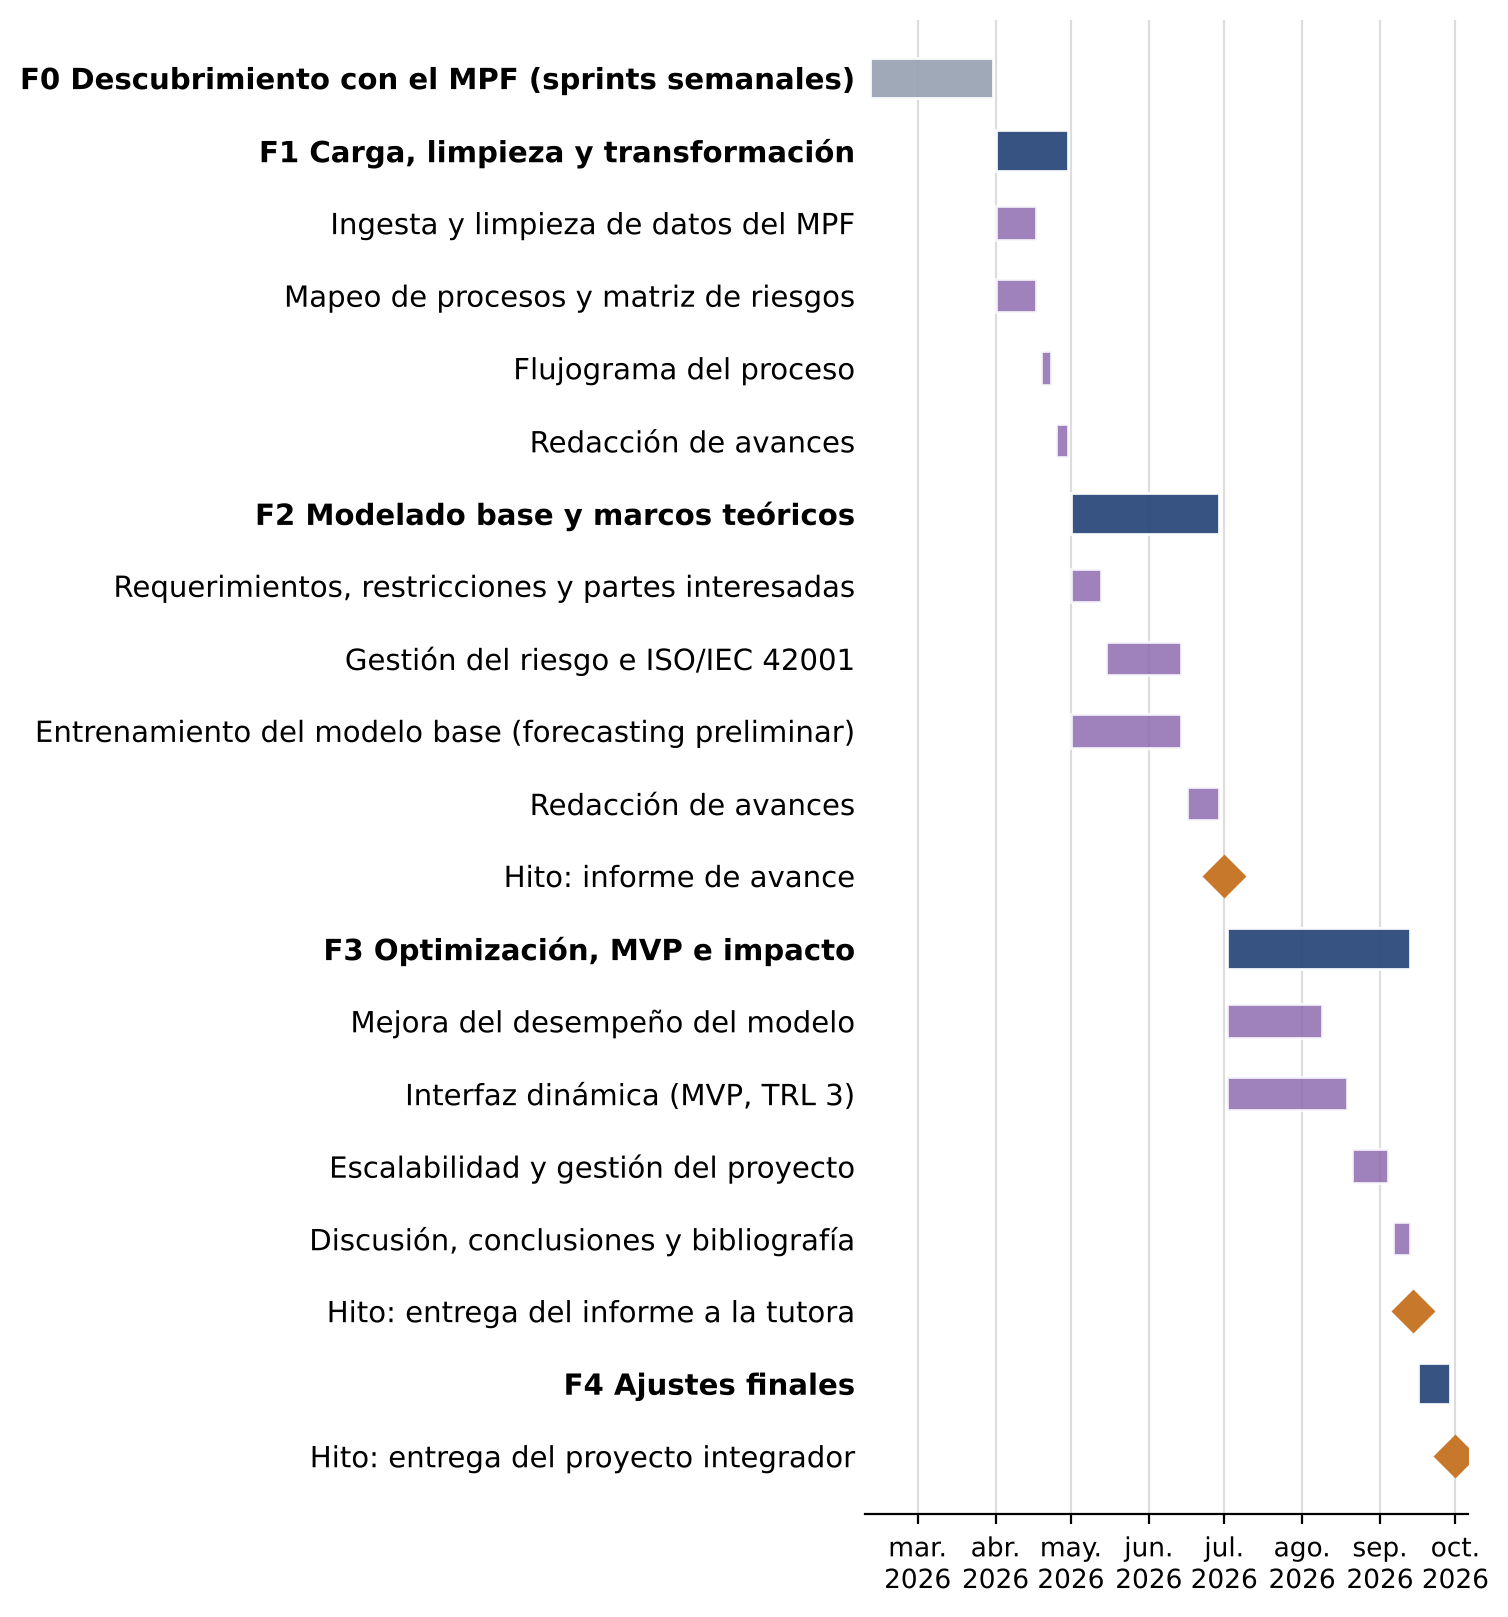
\includegraphics[width=\linewidth]{imagenes/gantt_proyecto.png}
\caption{Cronograma del proyecto integrador}
\label{fig:gantt-proyecto}
\notaflot{\fuentepropia. La fase F0 corresponde a la etapa de descubrimiento; las fases F1 a F4 y sus tareas reproducen el cronograma planificado para la etapa de ejecución.}
\end{figure}

\section{El Problema}\label{el-problema}

Como se mencionó en las etapas introductorias de este proyecto el punto central del problema que se intenta resolver es la gran demanda a la que se enfrenta todos los días el personal del MPF en términos de toma de decisiones para la gestión de tareas y recursos. Los accidentes viales son eventos que tienen escasa probabilidad de suceder en comparación con otros eventos que también gestiona el Ministerio Público Fiscal, sin embargo tienen una característica que los distingue en gran medida de estos últimos, y es que genera un gran impacto a nivel demanda de recursos. En este tipo de eventos es importante destacar que tal demanda no es uniforme, es decir, dado que cada accidente tiene particularidades propias de la naturaleza del mismo dos de ellos pueden implicar tanto distinta cantidad como distinto recurso propiamente dicho. A esto debe agregarse también el hecho de que la ventana de tiempo para asignar no solo es muy limitada en el tiempo si no que puede ser determinante en cuanto al proceso penal. Entrando específicamente en qué recursos se deben gestionar se puede destacar tanto el personal principal propio del MPF como lo pueden ser, oficiales de justicia, peritos especializados, la policía, como terceros pero fuertemente vinculados como el personal de tránsito, funcionarios municipales, y personal de clínicas y hospitales.

Se tiene así entonces un problema de gran complejidad, que surge de la combinación de tres aspectos y características fundamentales. El proceso es altamente demandante a nivel coordinación de personal y recursos técnicos, también es imprescindible hacerlo con la máxima velocidad y precisión porque está vinculado al posible proceso penal y por último es un evento que hasta ahora era impredecible por lo que el MPF está obligado a sobre dimensionar sus operaciones referidas a accidentes viales. Queda de esta manera definido el principal punto de dolor del usuario siendo esto la motivación principal de este proyecto.

Teniendo en cuenta lo anteriormente expuesto sería posible intuir que una forma de solucionarlo pueda ser el uso de tecnología, pero esto es parcialmente cierto. Desde el punto de vista de la ingeniería industrial este problema debe considerar el enfoque de personas, procesos y tecnología (PPT) el cual sugiere que estos tres aspectos son los factores clave que hay que gestionar para solucionar el problema de la forma apropiada.

Si se analiza la dimensión de las personas se debe destacar que el dominio de los usuarios tiene limitaciones determinantes en cuanto a conocimiento específico de herramientas de software o modelos estadísticos avanzados, esto sin duda impacta en cómo se diseñará el producto en términos de explicabilidad y experiencia de usuario. En lo referido a los procesos se destaca especialmente la disponibilidad de información en bloques agregados y el poco volumen de datos existentes. Finalmente en la dimensión tecnológica se debe tener en cuenta aspectos de seguridad informática, normativas, limitarse al uso de tecnología de código abierto, escalabilidad, y mantenimiento de la misma a largo plazo. La conjunción de estos tres aspectos generará una serie de opciones y alternativas para seleccionar las mejores tecnologías que se adapten a los procesos que protagonizan las personas.

Recientemente se mencionó que el problema estaba definido por tres características fundamentales, es altamente demandante en recursos, requiere velocidad y precisión, y es difícil anticipar en qué momentos se concentrará la demanda de ese proceso. Es en este último punto donde se decidió diseñar un sistema de alerta temprana basado en \eng{forecasting} e impulsado por inteligencia artificial, con la hipótesis de que prever con cierto grado de anticipación cuando hay más riesgo de ocurrencia de accidentes viales puede aportar información útil para planificar las operaciones del MPF.


\section{Objeto y requerimientos del sistema}\label{sec:objeto-requerimientos}

Esta sección sigue la secuencia objeto, relevamiento y requerimientos: primero se define qué es el sistema y para quién, después cómo se relevaron sus requerimientos y por último cuáles son.

\subsection{Objeto del sistema}\label{ssec:objeto}

El objeto del sistema es estimar, para cada bloque de seis horas, el riesgo de que ocurra en la ciudad de Córdoba al menos un siniestro vial con víctimas, y comunicar ese riesgo como una alerta comprensible para el personal del área de Accidentología Vial del Ministerio Público Fiscal, de modo que pueda anticipar la asignación de sus recursos.

El sistema está destinado exclusivamente a ese personal. Dado que el Ministerio Público Fiscal tiene una cantidad significativa de áreas con distintas responsabilidades y roles, es válido aclarar para quién no es este producto: no está destinado al personal de Policía Judicial, a los agentes de tránsito, al personal municipal, al personal que no corresponda a Accidentología Vial ni a la ciudadanía en general. Las partes interesadas, en el sentido de la cláusula 4.2 de ISO/IEC 42001, son el Ministerio Público Fiscal, el área de Accidentología Vial del MPF, el área de Formación del MPF, LIDeSIA y la FCEFyN.

\subsection{Relevamiento de requerimientos}\label{ssec:relevamiento}

No existió un documento de requerimientos previo. Los requerimientos se relevaron a partir de cuatro fuentes:

\begin{itemize}[itemsep=2pt]
  \item las reuniones semanales de la etapa de descubrimiento con el representante de la Unidad Judicial y la directora de LIDeSIA (\cref{ssec:descubrimiento}), principal fuente de información sobre el proceso, los usuarios y la forma de comunicar el riesgo;
  \item las pruebas de usuario del sistema de gestión de siniestros realizadas durante las prácticas profesionales supervisadas de los autores, que pusieron en evidencia la necesidad de incorporar capacidades predictivas (\cref{surgimiento-del-proyecto});
  \item el análisis documental de la base de datos, de su diccionario de variables y del procedimiento judicial (\cref{procedimiento-judicial-ante-un-siniestro,los-datos});
  \item las normas adoptadas como referencia, en particular los apartados A.6.2.2 y B.6.2.2 de ISO/IEC 42001 sobre requerimientos y especificación del sistema de IA.
\end{itemize}

Cada requerimiento surgido de estas fuentes se registró como tarea en el tablero del proyecto y se validó en la reunión de revisión siguiente.

\subsection{Requerimientos}\label{ssec:requerimientos}

La \cref{tab:requerimientos} reúne los requerimientos funcionales y no funcionales relevados, junto con su estado al cierre de este trabajo. Los requerimientos que quedan pendientes forman parte del plan de implementación del \cref{cap:implementacion}. % C6.8: frase marcada para revisar; decidir si se mantiene.

{\setstretch{1.0}\small
\begin{longtable}{@{}>{\raggedright\arraybackslash}p{0.08\textwidth}
                    >{\raggedright\arraybackslash}p{0.44\textwidth}
                    >{\raggedright\arraybackslash}p{0.21\textwidth}
                    >{\raggedright\arraybackslash}p{0.19\textwidth}@{}}
\caption{Requerimientos del sistema}
\label{tab:requerimientos} \\
\toprule
\textbf{ID} & \textbf{Requerimiento} & \textbf{Fuente} & \textbf{Estado (TRL~3)} \\
\midrule
\endfirsthead
\multicolumn{4}{@{}l}{\footnotesize\textit{Tabla \ref{tab:requerimientos} (continuación)}} \\
\toprule
\textbf{ID} & \textbf{Requerimiento} & \textbf{Fuente} & \textbf{Estado (TRL~3)} \\
\midrule
\endhead
\bottomrule
\endfoot
\multicolumn{4}{@{}l}{\textit{Funcionales}} \\
RF1 & Transformar la base de siniestros del MPF en una serie continua agregada en bloques de seis horas. & Reuniones con el MPF & Cumplido \\
RF2 & Estimar para cada bloque el riesgo de al menos una víctima. & Necesidad del MPF & Cumplido \\
RF3 & Traducir la estimación en una alerta mediante una capa de decisión. & Reuniones con el MPF & Cumplido (binaria) \\
RF4 & Expresar la alerta en una escala de tres colores. & Reuniones con el MPF & Especificado \\
RF5 & Permitir ajustar los umbrales sin reentrenar el modelo. & Riesgo de fatiga de alertas & Cumplido \\
RF6 & Informar qué variables explican la predicción. & ISO/IEC 42001, A.8.2 & Cumplido (global) \\
RF7 & Registrar cada alerta emitida y la decisión humana adoptada. & Riesgo R7 & Pendiente \\
\midrule
\multicolumn{4}{@{}l}{\textit{No funcionales}} \\
RNF1 & Utilizar modelos explicables (XAI). & ISO/IEC 42001 & Cumplido \\
RNF2 & Utilizar exclusivamente tecnología de código abierto. & LIDeSIA & Cumplido \\
RNF3 & Alojar el servicio y el entrenamiento en la infraestructura del CCAD. & LIDeSIA & Cumplido (entrenamiento) \\
RNF4 & Trabajar solo con datos anonimizados (Ley N.º 25.326). & Convenio MPF--LIDeSIA & Cumplido; R4 pendiente \\
RNF5 & Presentar la información en un formato comprensible para usuarios sin formación estadística. & Reuniones con el MPF & Especificado \\
RNF6 & Garantizar una disponibilidad acorde a un servicio de 24 horas. & Proceso judicial & Pendiente \\
RNF7 & Contar con control de acceso basado en roles y medidas de ciberseguridad. & ISO/IEC 42001 & Pendiente \\
\end{longtable}
}
\notaflot{\fuentepropia. «Especificado» indica que el requerimiento quedó definido pero no se implementó en la prueba de concepto.}

Los requerimientos se apoyan en una serie de supuestos sobre las restricciones que imponen los modelos para series temporales. Un algoritmo que predice el riesgo de accidentes viales necesita información en bloques discretos de tiempo, es decir que se requiere que los usuarios finales mantengan permanentemente actualizados los datos que son entrada del modelo. En este proyecto los bloques de predicción son de seis horas, por lo que es necesario poder agregar todos los datos conocidos en ese intervalo para realizar la predicción. Existen otros modelos más flexibles respecto de esta restricción, pero el requerimiento de explicabilidad (RNF1) obliga a seleccionar un modelo explicable. Se asume entonces esta restricción y se da por supuesto que el equipo del MPF se compromete a mantener los datos actualizados.

El alcance definido para la gestión de este proyecto es el de un producto mínimo viable. Si bien no se implementan todas las características funcionales y no funcionales (control de acceso basado en roles, cumplimiento de todos los puntos de la norma ISO/IEC 42001, ciberseguridad, diseño de la experiencia de usuario), el diseño las contempla para que puedan incorporarse sin generar incompatibilidades.

En cuanto a la necesidad de realizar \eng{forecasting}, se justifica bajo el apartado B.6.2.2 de ISO/IEC 42001 (requerimientos y especificación del sistema de IA) como una evolución deseable del sistema de gestión descriptivo existente, que permite pasar de la caracterización a la predicción. La especificación funcional de la capa de decisión (RF4) se traduce en una escala de tres niveles basada en el puntaje estándar Z-Score: alerta roja si el riesgo predicho supera las dos desviaciones estándar respecto del promedio histórico, amarilla si se ubica entre una y dos desviaciones, y verde si el riesgo es menor o igual a una desviación estándar. % VERIFICAR: cortes de la escala de tres niveles.
Esta escala quedó especificada como diseño y no se evaluó en este trabajo.

\section{Los datos}\label{los-datos}

La correcta carga de datos es un aspecto clave para el funcionamiento del sistema: introducir información errónea o planificar mal los datos que se van a tomar puede comprometer la integridad de todo el proyecto, anulando el valor de los análisis, realizando malas predicciones debido a información errónea y condicionando a futuro todo el ciclo de vida del producto.

Entonces, los datos son recopilados por el personal del Ministerio Público Fiscal y cargados a la base de datos, pero aquí no terminan las responsabilidades del MPF ya que de acuerdo con el convenio de confidencialidad firmado entre el MPF y LIDeSIA, y en cumplimiento de la Ley N.º 25.326 de protección de datos personales el MPF suprimirá toda información sensible antes de hacer entrega de su base de datos de accidentología.

Una vez anonimizados, los datos llegan en formato de tabla de cálculo que cuenta con 8 agrupaciones de variables distintas para cada siniestro relevado, estas son: Información del sumario (Número de sumario, número de SAC, entre otras variables), Información básica del caso (fecha, hora, lugar, fiscal a cargo, ayudante de fiscal, entre otros), Datos de la persona denunciante o víctima (previamente anonimizados, edad, género, fecha de citación, entre otros), Datos de la persona denunciada o aprehendida (Ídem agrupación anterior más si tiene seguro y si se fugó), Información sobre objetos (descripción y observación de vehículos, si hay secuestro o resguardo, destino del mismo, fecha de informe, fecha de entrega, entre otros), Decisiones sobre el caso de fiscalía o juzgado (fecha de imputación, recupero de la libertad, decreto de detención, prisión preventiva y directivas de fiscalía, juzgado o ayudante de fiscal), Observaciones del caso (observaciones) y Remisión (Fecha de salida de la UJ, motivo y oficina a la que se la remite).

Lo mencionado anteriormente describe de forma rápida cómo se conforman los datos ``crudos'' que llegan a LIDeSIA, éstos una vez recibidos son procesados por el equipo de datos. Este equipo inicia su labor consolidando registros de diversos años y estructurándolos en niveles diferenciados para hechos y personas, corrigiendo duplicados de expedientes SAC mediante una codificación especial. Tras este paso, realizan una lectura manual de más de \num{9000} registros para identificar vehículos y tipos de siniestros, e implementan una geocodificación individual en Google Maps que descarta casos con ubicaciones imprecisas fuera de la ciudad. El proceso continúa con el enriquecimiento de la base mediante datos astronómicos externos para definir la iluminación solar y el cálculo de distancias radiales a elementos críticos de infraestructura como semáforos, esquinas y luminarias. Finalmente, transforman los datos en variables binarias de presencia/ausencia y recategorizan medidas en cuartiles, entregando una planilla unificada con múltiples hojas y diccionarios técnicos listos para diversos análisis estadísticos.

Una vez procesados por el equipo de datos, quedan en existencia más de 110 variables únicas en total, distribuidas en distintas pestañas de la hoja de cálculo que es entregada a los autores. Es importante notar que muchas de estas variables son en realidad la misma información presentada en diferentes formatos (texto, código numérico, categorías o cuantiles) para facilitar distintos tipos de procesamiento estadístico.

A modo explicativo, se presenta una lista de la mayoría de estas variables y su explicación diferenciadas en 5 grandes grupos.

\begin{longtable}[]{@{}
>{\raggedright\arraybackslash}p{(\linewidth - 2\tabcolsep) * \real{0.3594}}
  >{\raggedright\arraybackslash}p{(\linewidth - 2\tabcolsep) * \real{0.6032}}@{}}
\caption{Resumen de variables del dataset original}
\label{tab:resumen-de-variables-del-dataset-origina}\\
\toprule\noalign{}
\textbf{Nombre} & \textbf{Contenido} \\
\midrule\noalign{}
\endfirsthead
\toprule\noalign{}
\textbf{Nombre} & \textbf{Contenido} \\
\midrule\noalign{}
\endhead
\bottomrule\noalign{}
\endlastfoot
\multicolumn{2}{@{}>{\raggedright\arraybackslash}p{(\linewidth - 2\tabcolsep) * \real{0.9626} + 2\tabcolsep}@{}}{%
\textbf{Grupo 1: Identificadores y Datos Generales}} \\
Nro. de SAC / id\_caso & Identificador único del siniestro basado en el número de expediente judicial. \\
Fecha de ingreso & Fecha en que se registró el expediente en el sistema. \\
Lugar\_hecho & Domicilio y referencia espacial donde ocurrió el siniestro. \\
Lesiones / Lesionescod & Descripción y código del tipo de lesiones (leves, graves, homicidio u otras). \\
Cant\_lesionados & Cantidad total de personas que resultaron heridas en el hecho. \\
\multicolumn{2}{@{}>{\raggedright\arraybackslash}p{(\linewidth - 2\tabcolsep) * \real{0.9626} + 2\tabcolsep}@{}}{%
\textbf{Grupo 2: Variables Temporales}} \\
Hora del hecho / hora\_hecho & Horario real del siniestro registrado en formato de 24 horas. \\
Franja\_horaria / horacod2 & Clasificación del horario en periodos (madrugada, mañana, etc.) o intervalos de movilidad. \\
Día\_semana\_cat & Representación numérica del día de la semana (1-Lunes a 7-Domingo). \\
Mes / TIPOMESCOD & Mes del año y su clasificación según el ciclo lectivo (escolar o no escolar). \\
Es\_fin\_de\_semana / FINDECOD & Variable que indica si el siniestro ocurrió en sábado o domingo. \\
EstacionCLIMA / Estación & Indica la estación del año (otoño, invierno, primavera, verano). \\
Es\_hora\_punta & Indica si el hecho ocurrió en horarios de alta congestión (ingreso/egreso laboral y escolar). \\
Variables Solares & Datos sobre amanecer, salida del sol, mediodía, anochecer y puesta del sol para cada día. \\
Horasxdia & Cantidad total de horas de luz solar que tuvo la jornada del siniestro. \\
\multicolumn{2}{@{}>{\raggedright\arraybackslash}p{(\linewidth - 2\tabcolsep) * \real{0.9626} + 2\tabcolsep}@{}}{%
\textbf{Grupo 3: Datos de las Personas Involucradas}} \\
Cant\_involucrados / TotalPersonas & Número total de sujetos (víctimas y denunciados) participantes en el siniestro. \\
Víctimas / Denunciados & Conteo específico de personas afectadas y de presuntos responsables por cada hecho. \\
Desglose por Sexo & Cantidad de víctimas y denunciados (femeninos y masculinos) por siniestro. \\
Grupos Etarios & Cantidad de niños, jóvenes, adultos y adultos mayores según rangos de la OMS. \\
Estadísticas de Edad & Valores descriptivos: edad media, mínima, máxima y mediana de los involucrados. \\
Género\_predominante & Identifica cuál es el género con mayor representación en el evento. \\
Sin\_datos\_edad / genero & Cantidad de personas involucradas de las que se desconoce su edad o género. \\
\multicolumn{2}{@{}>{\raggedright\arraybackslash}p{(\linewidth - 2\tabcolsep) * \real{0.9626} + 2\tabcolsep}@{}}{%
\textbf{Grupo 4: Vehículos e Infraestructura}} \\
Vehículo 1 / Vehículo 2 & Identificación y tipo de las unidades motorizadas involucradas en la colisión. \\
TOTAL\_VEHICULOS & Cantidad total de vehículos participantes en el siniestro. \\
Tamaño1 / Tamaño2 & Clasificación según el peso aproximado (persona, ligero, mediano, medio pesado o pesado). \\
Motorizado / Transporte público & Indica si el vehículo tiene motor o si pertenece al sistema de transporte masivo. \\
Inmovil & Indica si el impacto fue contra un objeto fijo (árbol, poste, pared, etc.). \\
TipoVÍA / TIPOVIA2 & Clasificación de la calle según su jerarquía vial (arterial, sectorial o de barrio). \\
Enesquina & Determina si el hecho ocurrió a 15 metros o menos de una intersección. \\
Distancia Semáforo / Luminaria & Distancia radial en metros al dispositivo de control o luz más cercana. \\
Dianoche & Clasifica el siniestro como diurno o nocturno según luz solar real. \\
LUMI\_NOCHE & Indica si había luz artificial activa en siniestros ocurridos fuera del horario solar. \\
\multicolumn{2}{@{}>{\raggedright\arraybackslash}p{(\linewidth - 2\tabcolsep) * \real{0.9626} + 2\tabcolsep}@{}}{%
\textbf{Grupo 5: Procesamiento Estadístico y Recategorización}} \\
Variables de Presencia & Indicadores binarios (Sí/No) para factores como seguro, fuga, peatón, moto o bicicleta. \\
Cuartiles de Edad & Recategorización de las edades en cuatro grupos estadísticamente proporcionales. \\
Clústeres (temp, pers, mixto) & Agrupamientos estadísticos creados para identificar patrones comunes en los siniestros. \\
Distcentrocod & Categorización de la distancia al centro de la ciudad en rangos (ej. menos de 5 km). \\
Cantidades recategorizadas & Transformación de valores numéricos de involucrados o vehículos en categorías grupales. \\
Casospad & Columna técnica de referencia para el control de integridad durante el procesamiento. \\
\end{longtable}

\notaflot{\fuentepropia{}.}

\section{Exploración de datos}\label{exploraciuxf3n-de-datos}

La base utilizada en este trabajo proviene del registro de siniestros viales de la Unidad Judicial de Accidentología Vial del Ministerio Público Fiscal de Córdoba, al que se accedió en el marco de la colaboración con LIDeSIA. El archivo fuente, denominado \enquote{Siniestros unificados para nuevas variables}, se recibió acompañado de su documento de descripción y diccionario de variables. La totalidad de los registros fue anonimizada previamente a su entrega, en cumplimiento de la Ley N.º 25.326 de Protección de los Datos Personales, y durante todo el procesamiento se mantuvo el criterio de no incorporar ningún dato identificatorio de las personas involucradas.

El archivo original no constituye una tabla plana, sino una estructura que combina información del hecho, de las víctimas, de los denunciados, de las personas intervinientes y de la georreferenciación del evento. Esta organización responde a la lógica del expediente judicial y no a la de un conjunto de datos de entrenamiento: un mismo siniestro puede generar varios registros según la cantidad de personas o vehículos involucrados.

La primera tarea de curación consistió en definir el hecho como unidad de análisis y consolidar el resto de los niveles en atributos asociados a ese hecho, evitando la duplicación de casos.

Sobre esa base consolidada se aplicaron los siguientes criterios de depuración:

\begin{description}
  \item[Selección de la ventana temporal.] Se conservaron los siniestros comprendidos entre julio de 2022 y junio de 2024, período en el que el registro presenta continuidad y criterios de carga homogéneos.
  \item[Filtro de georreferenciación.] Se retuvieron únicamente los casos con coordenadas válidas dentro del ejido municipal de la ciudad de Córdoba, condición necesaria tanto para el análisis espacial como para la trazabilidad del registro.
  \item[Descarte de variables con fuga de información.] Se identificaron y removieron aquellos campos administrativos cuyo valor solo se completa con posterioridad al hecho y que, de conservarse, habrían filtrado información del futuro hacia el conjunto de entrenamiento.
  \item[Normalización de categorías.] Se unificaron las etiquetas de tipo de vehículo, tipo de vía y carátula de la causa, y se explicitaron los casos sin dato como categoría propia en lugar de imputarlos.
\end{description}

El resultado de esta etapa es un conjunto de \textbf{4320 siniestros georreferenciados}, que constituye la base sobre la que se realizó el análisis exploratorio que se presenta en las \crefrange{fig:distribucion-de-siniestros-viales-por-me}{fig:mapa-de-calor-de-siniestros-viales-en-la}.

\begin{figure}[htbp]
\centering
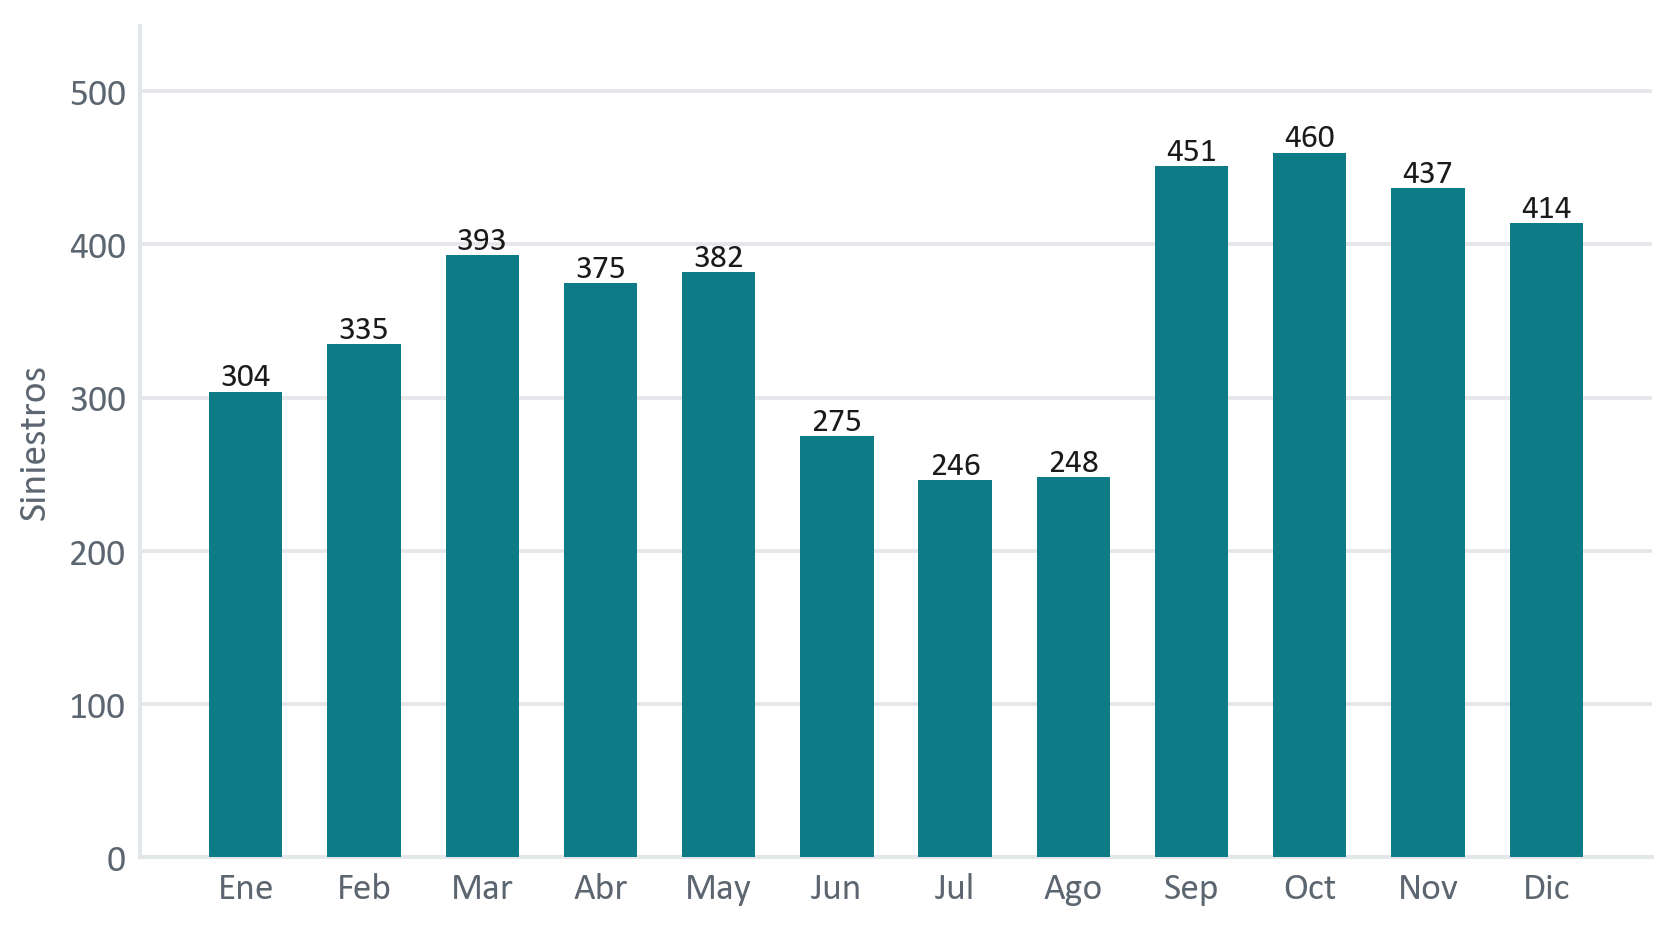
\includegraphics[width=0.92\linewidth]{imagenes/image2.png}
\caption{Distribución de siniestros viales por mes}
\label{fig:distribucion-de-siniestros-viales-por-me}
\notaflot{Frecuencia mensual acumulada de siniestros viales georreferenciados en la ciudad de Córdoba (n = 4320), julio 2022 -- junio 2024. El período de mayor concentración se ubica entre septiembre y diciembre, con un mínimo en julio y agosto. Julio computa únicamente 2023, y agosto 2022 y junio 2024 son meses parciales, por lo que esos tres meses acumulan menos años que el resto. \fuentepropia{} sobre la base de datos de la Unidad Judicial de Accidentología Vial.}
\end{figure}

\begin{figure}[htbp]
\centering
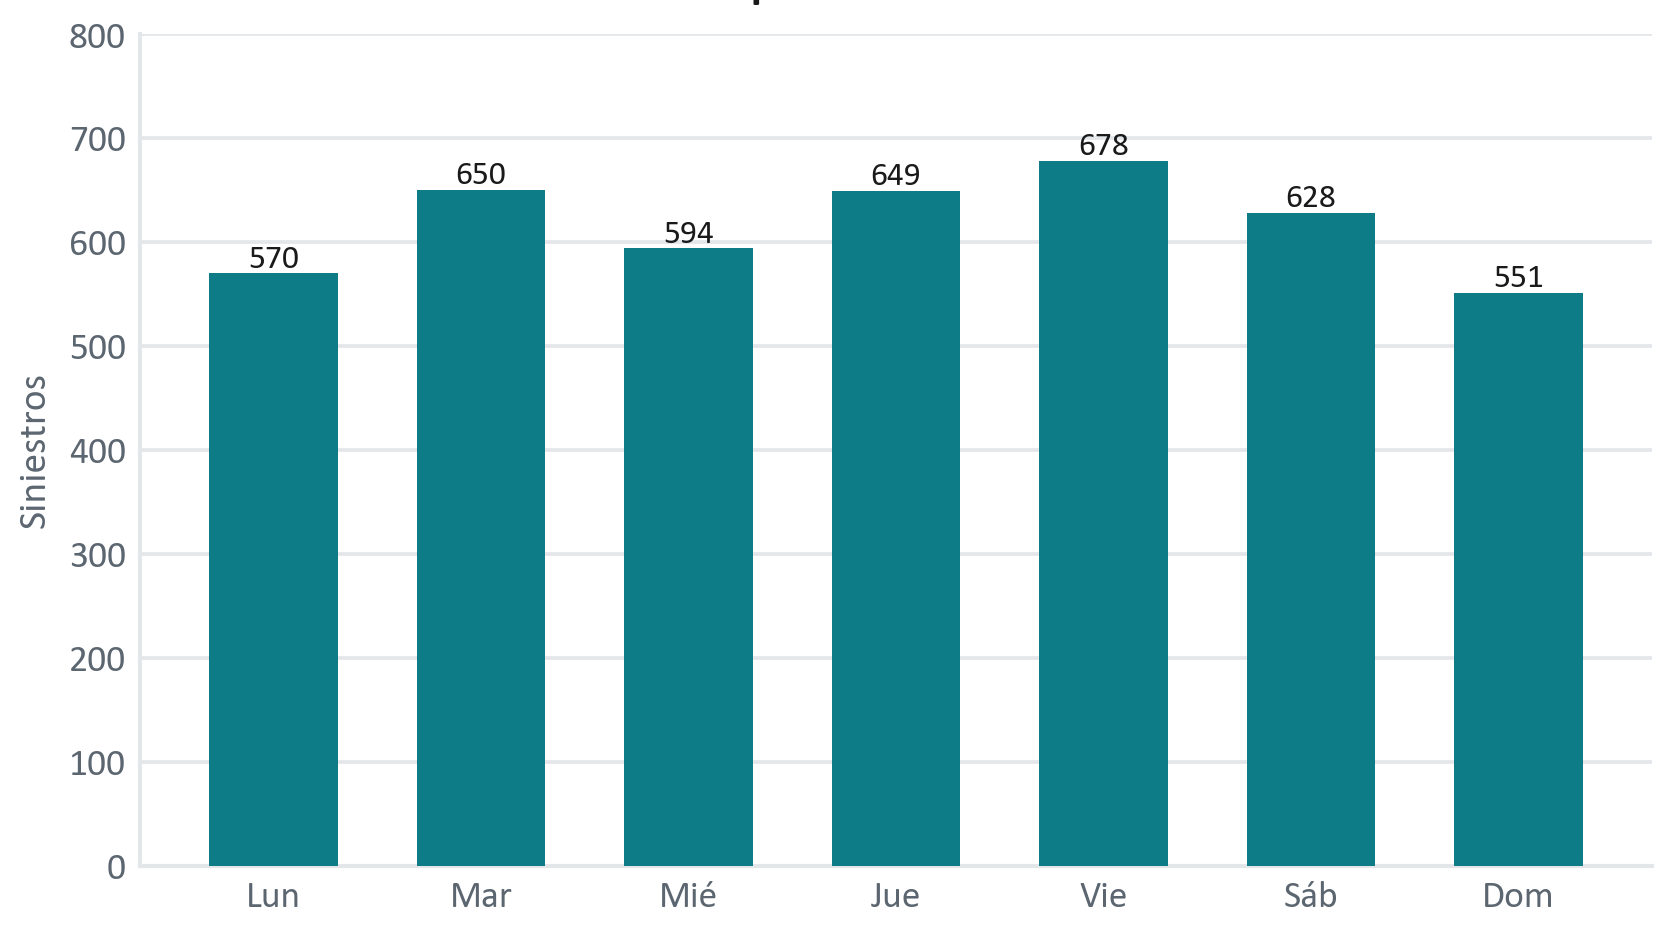
\includegraphics[width=0.92\linewidth]{imagenes/image1.png}
\caption{Distribución de siniestros viales por día de la semana}
\label{fig:distribucion-de-siniestros-viales-por-di}
\notaflot{Frecuencia de siniestros según día de la semana (n = 4320), julio 2022 -- junio 2024. La distribución es relativamente homogénea, con un máximo el viernes (678) y mínimos el domingo (551) y el lunes (570). \fuentepropia{}.}
\end{figure}

\begin{figure}[htbp]
\centering
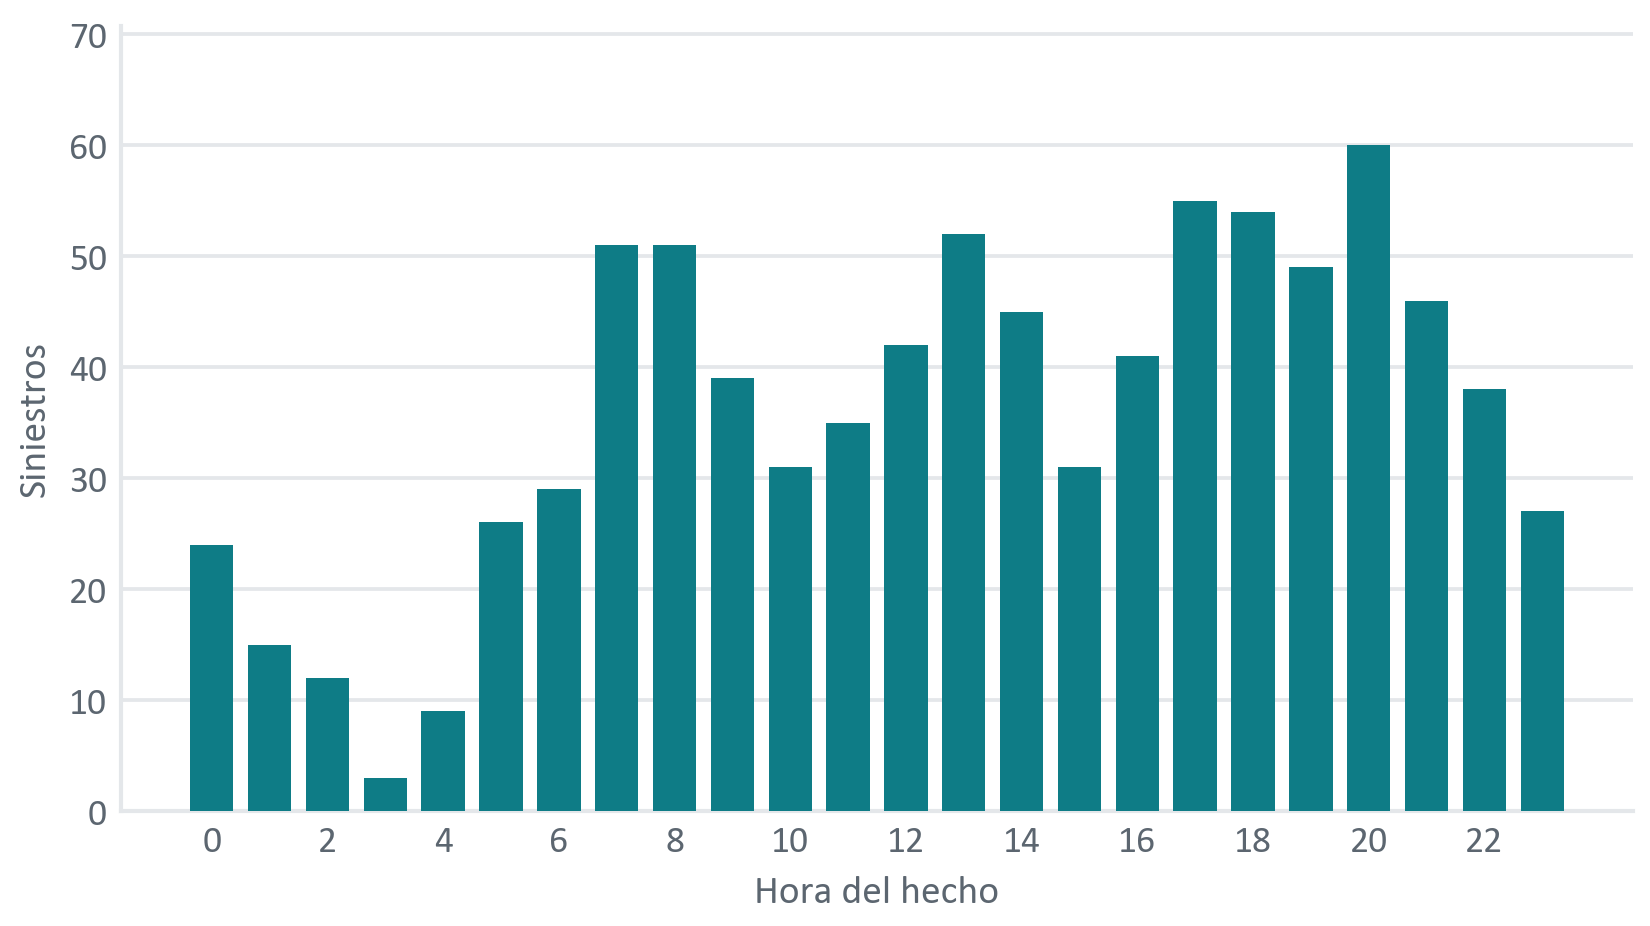
\includegraphics[width=0.92\linewidth]{imagenes/image6.png}
\caption{Siniestros viales por hora del día, año 2022}
\label{fig:siniestros-viales-por-hora-del-dia-ano-2}
\notaflot{Distribución horaria de los siniestros ocurridos durante 2022 (n = 865 registros con hora consignada; 23 casos sin dato, excluidos). Se identifican dos concentraciones asociadas a los desplazamientos cotidianos: una matutina (7 a 9 h) y otra vespertina, más prolongada e intensa (17 a 21 h), con el máximo absoluto a las 20 h. \fuentepropia{}.}
\end{figure}

\begin{figure}[htbp]
\centering
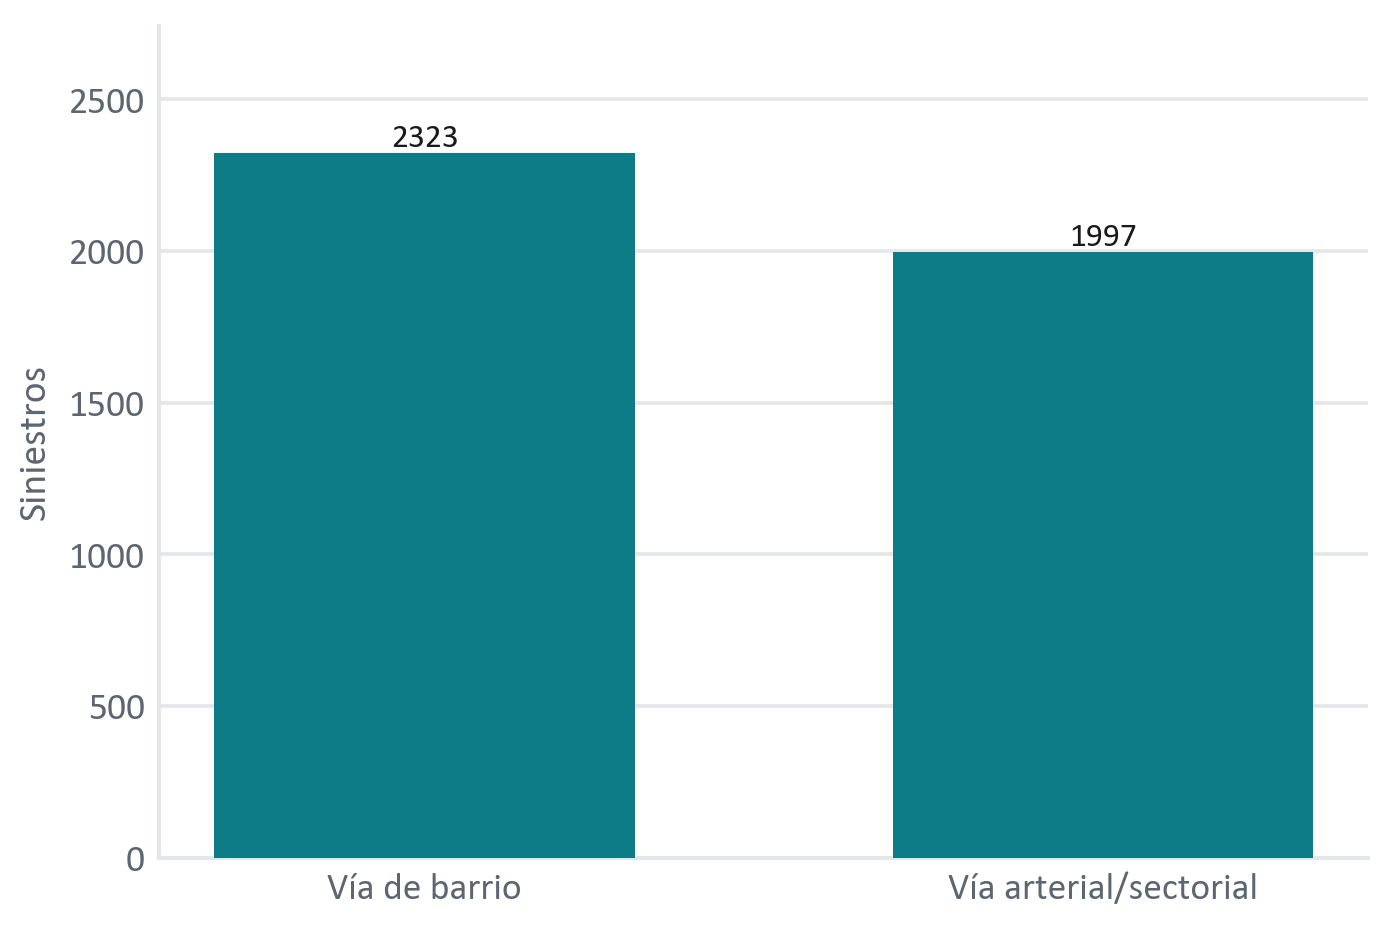
\includegraphics[width=0.78\linewidth]{imagenes/image3.png}
\caption{Distribución de siniestros viales por tipo de calle}
\label{fig:distribucion-de-siniestros-viales-por-ti}
\notaflot{Clasificación de los siniestros según jerarquía de la vía (n = 4320), julio 2022 -- junio 2024. Las vías de barrio concentran 2323 casos y las arteriales o sectoriales 1997, lo que muestra que el fenómeno no se restringe a los corredores principales. \fuentepropia{}.}
\end{figure}

\begin{figure}[htbp]
\centering
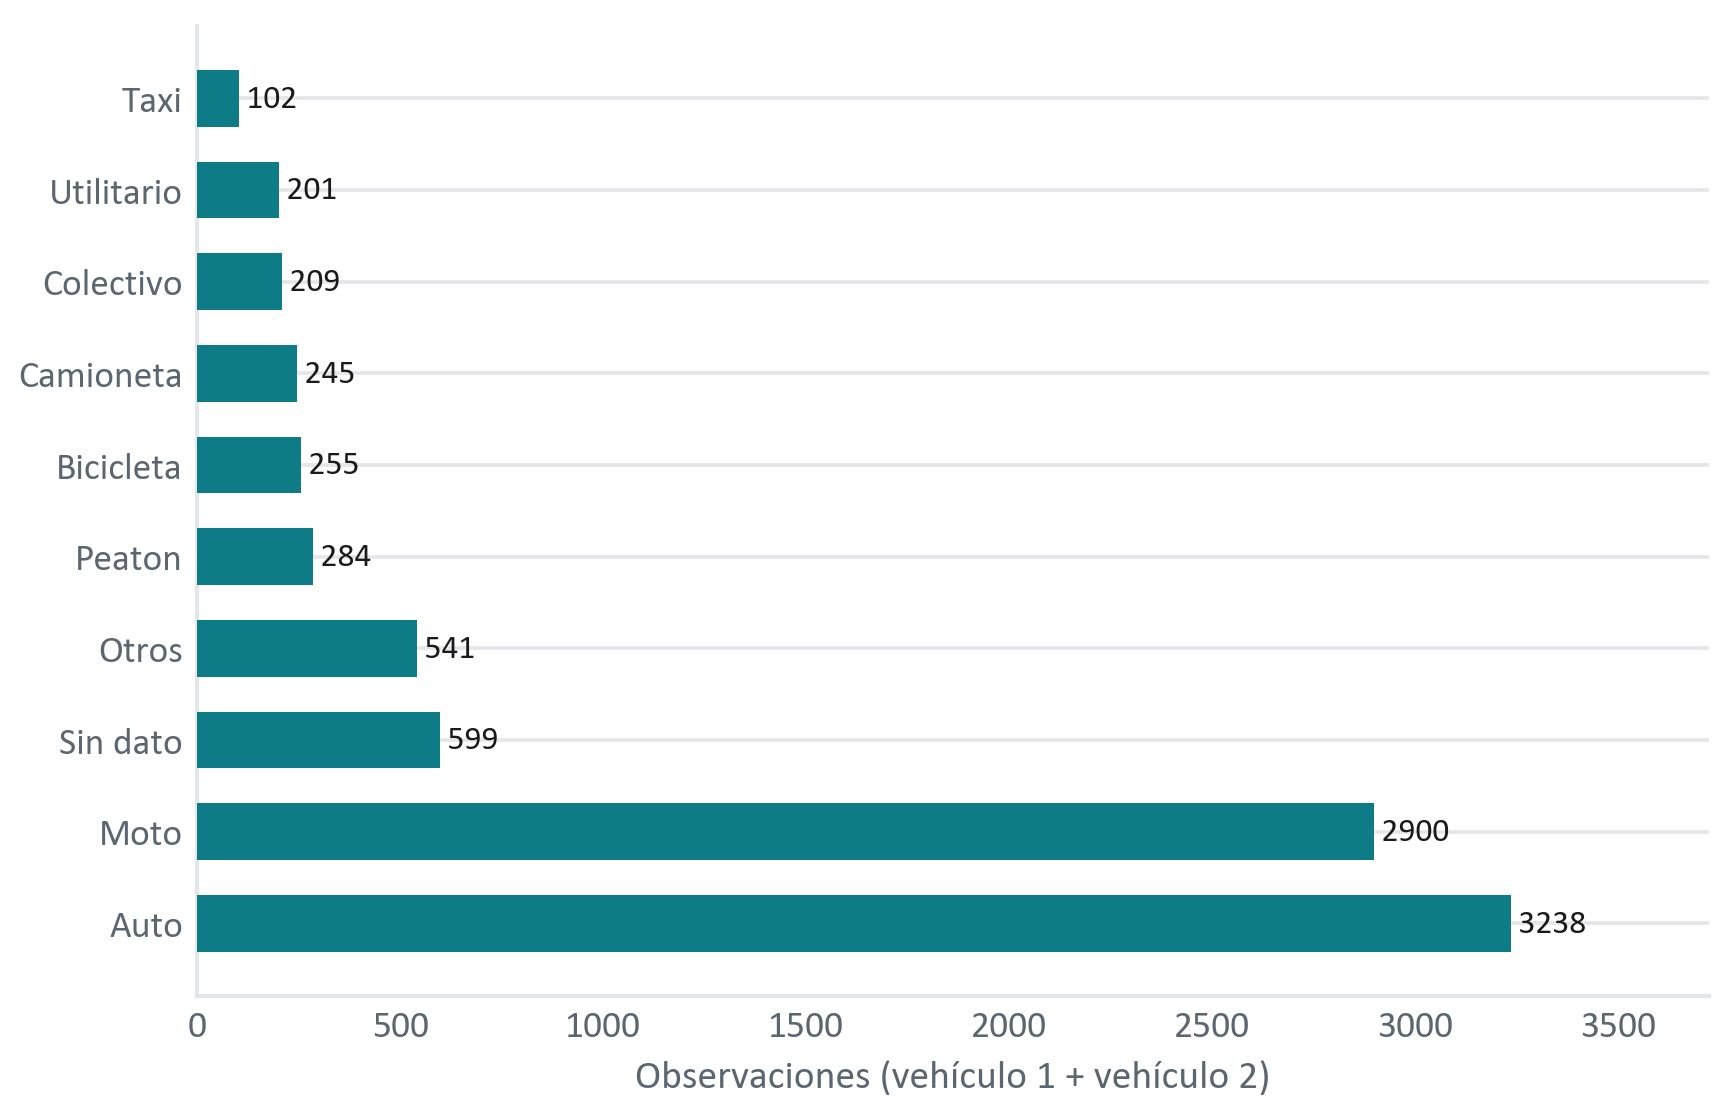
\includegraphics[width=0.81\linewidth]{imagenes/image16.png}
\caption{Distribución del tipo de vehículo o forma de desplazamiento}
\label{fig:distribucion-del-tipo-de-vehiculo-o-form}
\notaflot{Participaciones registradas en los 4320 siniestros (n = 8574 observaciones, correspondientes a vehículo 1 y vehículo 2). La unidad de conteo es la participación y no el siniestro, por lo que las categorías no son excluyentes entre sí. Autos (3238) y motos (2900) concentran la mayor parte de las observaciones. \fuentepropia{}.}
\end{figure}

\begin{figure}[htbp]
\centering
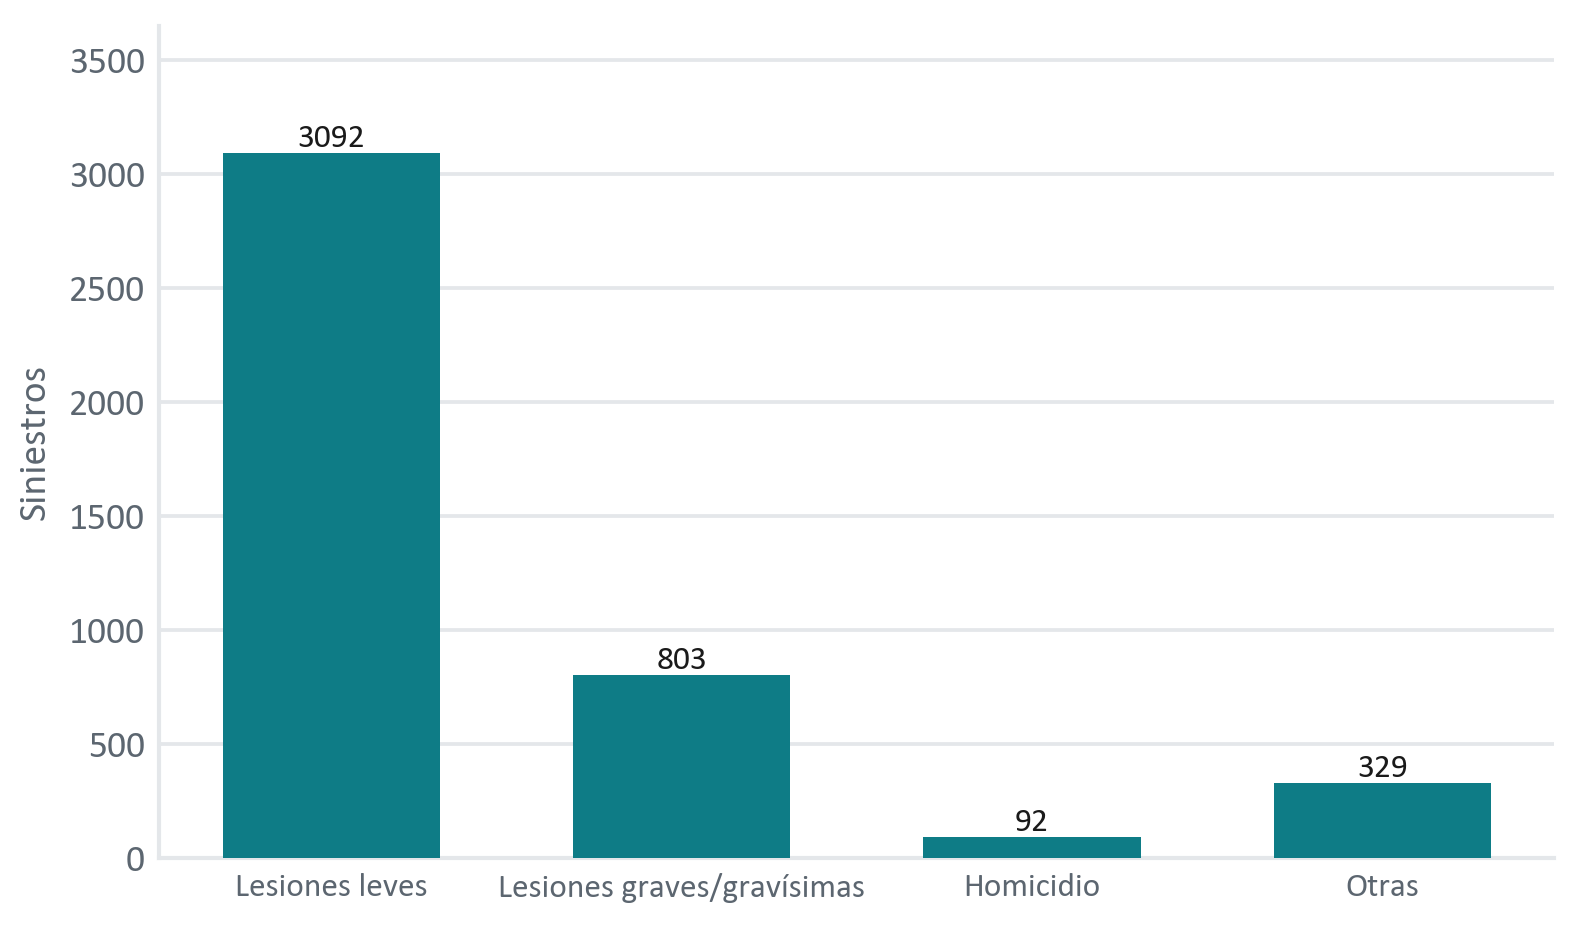
\includegraphics[width=0.89\linewidth]{imagenes/image5.png}
\caption{Distribución de siniestros viales según causa}
\label{fig:distribucion-de-siniestros-viales-segun-}
\notaflot{Clasificación de los siniestros según la carátula asignada en la causa judicial (n = 4316 casos clasificados; 4 sin clasificar, excluidos). Predominan las lesiones leves (3092), seguidas por lesiones graves o gravísimas (803), otras carátulas (329) y homicidio culposo (92). \fuentepropia{}.}
\end{figure}

\begin{figure}[htbp]
\centering
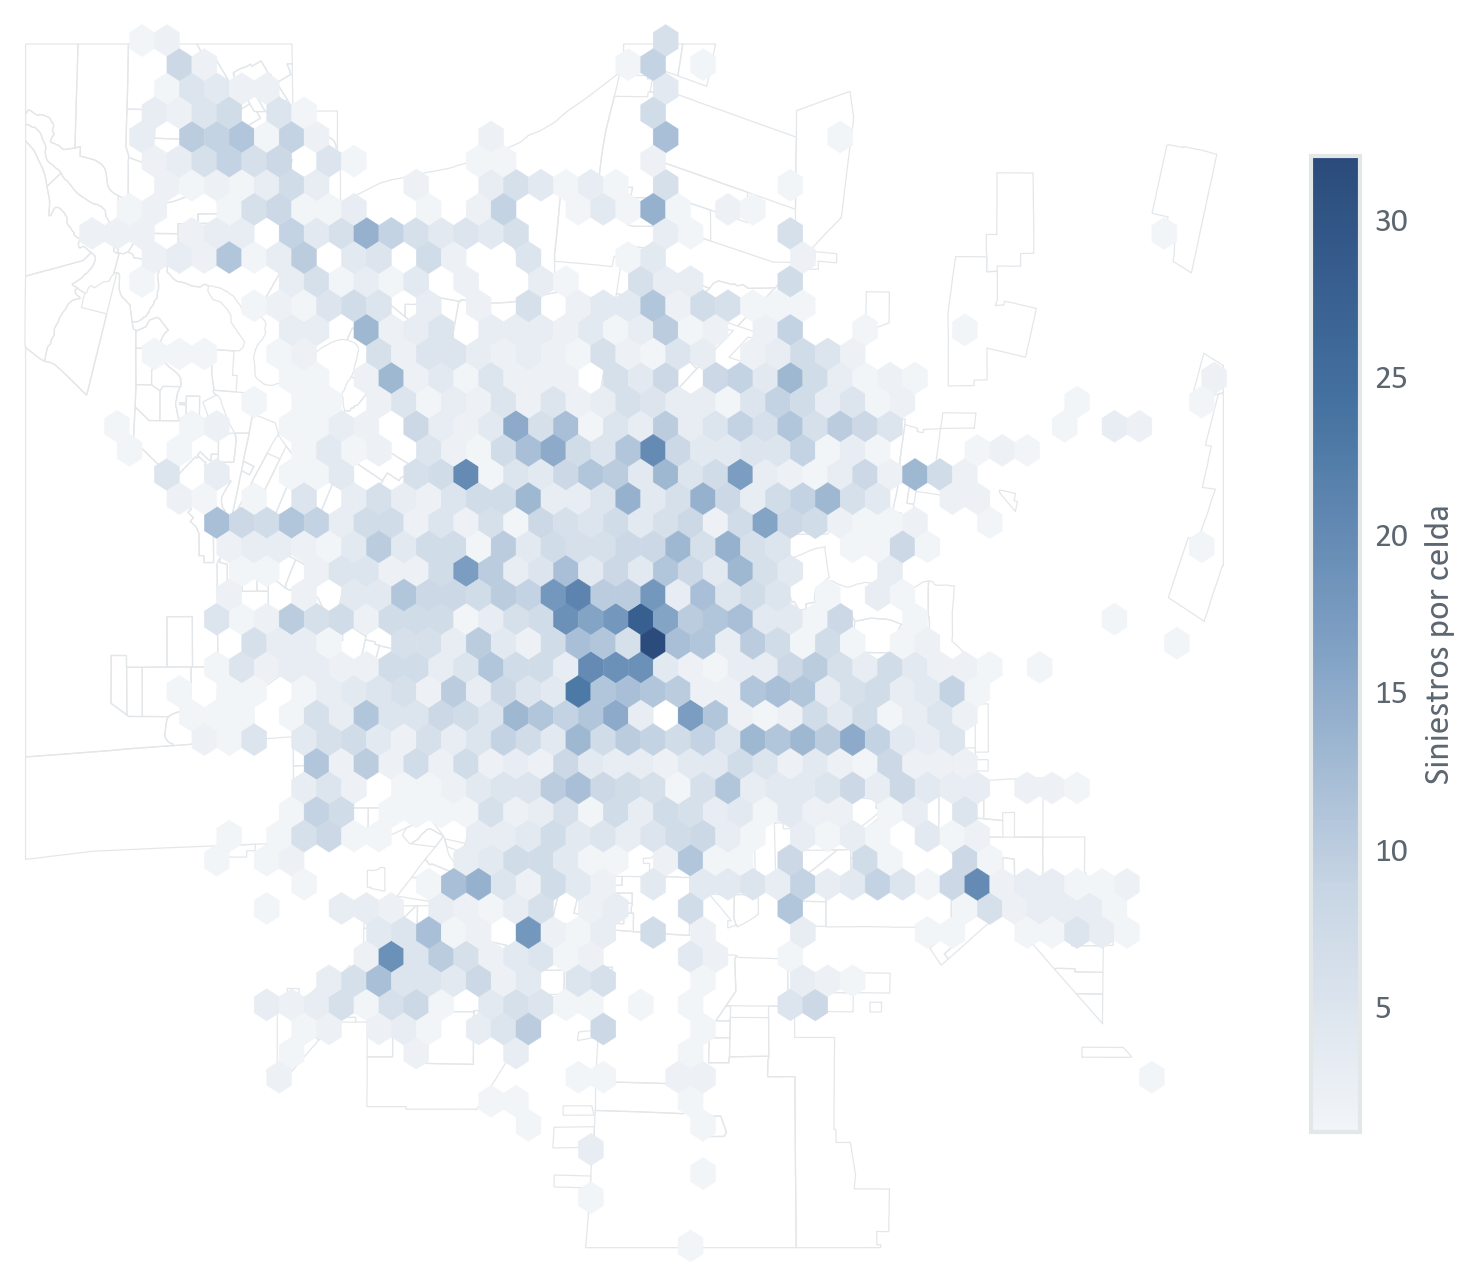
\includegraphics[width=0.92\linewidth]{imagenes/image8.png}
\caption{Mapa de calor de siniestros viales en la ciudad de Córdoba}
\label{fig:mapa-de-calor-de-siniestros-viales-en-la}
\notaflot{Densidad espacial de siniestros georreferenciados (n = 4320), julio 2022 -- junio 2024. La agregación se realiza por celda hexagonal de superficie constante y no por barrio; la silueta de los barrios se incluye solo como referencia visual. Se observa una concentración marcada en el área central y una difusión radial que sigue los principales corredores de acceso. \fuentepropia{}.}
\end{figure}

\section{Antecedentes Relevantes}\label{sec:antecedentes-relevantes}

Una de las tareas que se realizó inicialmente fue la investigación y la búsqueda de antecedentes relevantes, es decir trabajos o publicaciones que fueran sobre el mismo tema o que traten aspectos del enfoque, los datos y las técnicas de aprendizaje automático que sean transferibles o aplicables al producto que se está desarrollando. En este sentido se analizaron principalmente 4 grupos de antecedentes, trabajos sobre accidentología vial de índole analítica o basados en el uso de datos, \eng{forecasting} para problemas similares como incidentes con ambulancias o incendios, sistemas de alerta temprana, ciudades inteligentes, entre otros.

Independientemente del campo de aplicación en el cual se aplicaban los modelos revisados se observaron 3 tipos de enfoques posibles que describen a grandes rasgos las capacidades y requerimientos que se necesitan para un problema con accidentes viales. El primero consiste en trabajar con GNNs, un tipo de arquitectura de redes neuronales basadas en grafos que aprenden patrones de una gran cantidad de datos y que, al procesarlas en sus nodos, permiten generalizar el comportamiento de un sistema. El segundo se basa en el uso de datos georreferenciados. Independientemente del modelo específico utilizado, permite no solo predecir cuándo existe un mayor riesgo de accidentes, sino también dónde es más probable que ocurran. El último consiste en construir una tabla a partir de los registros de accidentes, donde una vez tratada para adaptar el set de datos para que represente una serie temporal se aplican modelos basados en árboles para aprender en qué contexto se incrementa el riesgo de accidentes.

Respecto de los modelos basados en grafos, fueron descartados rápidamente por varios motivos. Si bien se consiguen muy buenos resultados, todos los casos revisados tenían varios órdenes de magnitud adicionales en cantidad de datos, los cuales no eran solamente de accidentes sino que incluyen gran cantidad de variables externas como datos demográficos, información georreferenciada, datos de seguros, criminología, etc. Otra de las motivaciones para desistir por lo menos al inicio en desarrollar un modelo de esta complejidad era el de comenzar con un modelo más simple y si se conseguía buena capacidad de generalización avanzar en estos tipos de sistemas.

El antecedente más significativo para este proyecto es \textcite{novello2022}, que consiste en resolver el mismo problema utilizando inteligencia artificial sólo que aplicado en Ciudad Autónoma de Buenos Aires. La metodología consiste en usar datos georreferenciados y retardos para intentar predecir las zonas con riesgo más elevado. Este enfoque puede categorizarse como sistemas impulsados por modelos espacio-temporales. Respecto de este antecedente, si bien se decidió reproducirlo, hay que tener en cuenta un componente que es determinante para el resultado del mismo, esto es, la densidad de accidentes en el área de trabajo. Los datos para CABA totalizan \num{33234} registros de 29 características cada uno, distribuidos en 3,5 años y \qty{203}{\kilo\metre\squared} \parencite{novello2022}. Teniendo en cuenta la cantidad de registros para la Ciudad de Córdoba y el hecho de que tiene 2,8 veces más superficie (\qty{576}{\kilo\metre\squared}), la cantidad de accidentes por unidad de superficie es mucho menor por lo que el desempeño podría verse comprometido.

La última categoría mencionada es la de modelos tabulares basados en árboles. Generalmente requieren una menor cantidad de datos para alcanzar un buen desempeño que enfoques basados en redes neuronales profundas. Para esta metodología se encontró una cantidad considerable de trabajos, por lo que se deja como antecedente general el trabajo de \textcite{zheng2018} en su apartado sobre series temporales.


\section{Experimentación con Modelos}\label{experimentaciuxf3n-con-modelos}

Antes de seleccionar el modelo de línea base se realizó una serie de experimentos orientados a explorar distintos enfoques de predicción sobre un mismo fenómeno. Conviene advertir que esos modelos no son directamente comparables entre sí: cada uno fue construido bajo criterios y premisas propios, con formatos de salida distintos, de modo que sus métricas no admiten una lectura como un ranking de desempeño. El propósito de esta etapa no fue elegir un ganador por métrica, sino determinar qué manera de plantear el problema resulta más adecuada para un sistema de alerta temprana y qué enseñanzas deja cada intento sobre la naturaleza del fenómeno estudiado.

El detalle de cada experimento (configuración, métricas y figuras) se presenta en el \cref{ap:experimentos}. La \cref{tab:sintesis-experimentos} resume los seis enfoques evaluados y a continuación se exponen los hallazgos que condicionaron el diseño del producto.

\begin{table}[htbp]
\centering
\caption{Síntesis comparativa de los experimentos realizados}
\label{tab:sintesis-experimentos}
\begin{tabularx}{\linewidth}{@{}XXl@{}}
\toprule
\textbf{Experimento} & \textbf{Tipo de salida} & \textbf{Métrica principal} \\
\midrule
\lightgbm{} con intervalos P10--P90 & Regresión con cuantiles & MAE 0,9741 \\
Perceptrón multicapa clasificador & Clasificación en tres niveles & F1 ponderado 0,4327 \\
\xgboost{} regresor con capa Z-Score & Regresión más capa de decisión & RMSE 1,6966 \\
Perceptrón multicapa binario & Clasificación binaria con umbral & AUC-ROC 0,6289 \\
\xgboost{} georreferenciado & Clasificación espacio-temporal & PR-AUC 0,0097 \\
\autogluonts{} & Ensamble automatizado & MASE (Direct Tabular, 1.\textsuperscript{er} puesto) \\
\bottomrule
\end{tabularx}
\notaflot{Los modelos no son directamente comparables entre sí, dado que fueron construidos bajo distintos criterios y premisas y persiguen objetivos que, si bien siempre son predictivos, no comparten el formato de salida. La columna «Métrica principal» consigna el valor más representativo de cada enfoque y no constituye un ordenamiento de desempeño. \fuentepropia{}.}
\end{table}

\subsection{Resumen de Hallazgos en Experimentos}\label{resumen-de-hallazgos-en-experimentos}

El primer aspecto a considerar es cómo predecir la variable objetivo. Se trabajó con dos posibilidades: regresiones sobre la cantidad de víctimas y clasificaciones, tanto binarias como en varias categorías. Los hallazgos sugieren que a todos los modelos entrenados les cuesta identificar los momentos de bajo riesgo, independientemente de la forma de su salida. Es el caso del perceptrón multicapa en clasificación binaria, con un AUC-ROC de 0,6289, o del \xgboost{} de línea base, cuya sensibilidad en la clase normal es de 0,39 (identificó el \qty{38.5}{\percent} de los momentos en que no hubo siniestros con víctimas) frente a 0,87 en la clase crítica (\cref{pipeline-del-modelo-de-luxednea-base-baseline}). Entre los demás experimentos, el \lightgbm{} configurado con intervalos P10 y P90 fue el que mejor identificó los momentos seguros.

El segundo hallazgo es que, al comparar los modelos clasificadores con los regresores, resultó más adecuado para un sistema de alerta un esquema híbrido, compuesto por un modelo regresor y una capa de decisión que clasifique el riesgo después de la predicción. En este sentido se destaca el \xgboost{} regresor con capa Z-Score frente al perceptrón multicapa que clasifica directamente en alto, medio y bajo, que solo tiene un desempeño aceptable en una de sus clases.

Por último, a lo largo de toda la experimentación se confirmó, mediante entrenamientos con múltiples modelos y búsqueda por grilla de hiperparámetros, que el fenómeno se explica principalmente por el comportamiento reciente de la cantidad de víctimas y por algunas variables representativas del día de la semana y de la franja horaria. No se observaron contribuciones significativas a la capacidad predictiva de variables como la temperatura, la presión o el período escolar. Este aspecto se desarrolla en la sección de resultados del modelo de línea base.

\section{Pipeline del Modelo de Línea Base (Baseline)}\label{pipeline-del-modelo-de-luxednea-base-baseline}

Concluida la etapa experimental, se seleccionó \xgboost{} configurado como regresor de Poisson para constituir el modelo de línea base. El motivo es obtener un modelo que sirva de referencia para comparar y medir la evolución de futuros reentrenamientos, mejoras y adaptaciones, y también de cómo evoluciona la capacidad de predicción cuando se incorporan nuevos datos. La decisión se apoya en cuatro razones.

\begin{enumerate}[label=\alph*), leftmargin=2em, itemsep=2pt]
  \item \textbf{Convergencia de la evidencia experimental.} La búsqueda automatizada de \autogluonts{}, que evaluó cinco familias de modelos sin intervención sobre el criterio de selección, ubicó en primer lugar a Direct Tabular (implementación de modelos tabulares de árboles con ventanas deslizantes) por delante de DeepAR, AutoETS y TFT. Este resultado, obtenido de manera independiente, coincide con el de los experimentos manuales y con los antecedentes relevados en la \cref{sec:antecedentes-relevantes}.
  \item \textbf{Adecuación al volumen de datos disponible.} El conjunto cuenta con 2784 registros, una escala en la que los modelos basados en árboles suelen superar a las redes neuronales profundas. Los experimentos lo confirman: el perceptrón multicapa binario alcanzó un AUC-ROC de 0,6289 y la variante de tres clases un F1 ponderado de 0,4327, ambos por debajo del desempeño de las alternativas basadas en árboles.
  \item \textbf{Explicabilidad.} Al tratarse de un modelo construido sobre árboles de decisión, es posible extraer la contribución de cada variable a la predicción, lo que permite auditar el comportamiento del sistema y garantizar la explicabilidad, en línea con la norma ISO/IEC 42001. Las redes neuronales evaluadas no ofrecen esa trazabilidad de forma directa.
  \item \textbf{Aislamiento de la capacidad predictiva.} Configurar el modelo como regresor de Poisson con un umbral fijo permite medir su desempeño con independencia de las capas de decisión posteriores. Si la línea base incorporase la capa Z-Score, las mejoras registradas en futuros reentrenamientos no podrían atribuirse con claridad al modelo o a la calibración de los umbrales.
\end{enumerate}

Usualmente se trabaja con un modelo de complejidad relativamente baja respecto de otras técnicas, con el objetivo de experimentar rápidamente y testear hipótesis que permitan confirmar si los datos tienen la calidad y la cantidad suficientes \parencite{zheng2018} para que un determinado modelo adquiera una capacidad de generalización útil para el fin en cuestión.

Los aspectos analizados en la exploración de datos son de gran valor para comprender el problema: el conjunto es lo suficientemente específico, amplio en cantidad de características y adecuado para aplicar modelos de distintos tipos, como clasificadores que busquen patrones en grupos o modelos de analítica descriptiva más clásicos. Esto es posible porque el conjunto de datos contiene mucha información que caracteriza cada hecho en particular, como el tipo de vehículo involucrado, datos sobre las personas, la distancia al semáforo más próximo o la georreferenciación.

Sin embargo, la forma en la que esta información está estructurada no es útil para un sistema que pretende anticipar en una ventana de tiempo la cantidad de víctimas que pudiera haber. Cuando se trabaja con series temporales se utiliza información disponible en el momento o del pasado para realizar la predicción, pero en todos los casos tiene que ser información disponible antes del suceso que se quiere pronosticar. El formato de los datos originales se denomina tabla de hechos: cada fila es el registro de un hecho puntual en un determinado momento, con la fecha y la hora y, en las columnas siguientes, la información relevante del evento.

Uno de los principales aspectos que debió reformularse al inicio del proyecto deriva de la propia naturaleza de la tabla de hechos, que no registra el tiempo de manera continua: de los días en los que no hay accidentes no se tiene información. Esto es especialmente relevante para diseñar una alerta temprana, dado que es de vital importancia saber bajo qué condiciones no ocurren accidentes. Para resolverlo se dividió cada día en bloques de seis horas, de manera que los accidentes de un mismo bloque se suman para representar su riesgo y, cuando no hay accidentes, el bloque contiene un cero para indicarle al modelo que no ocurrió nada. Las demás variables se agregan según criterios convenientes para representar lo mejor posible a cada bloque; por ejemplo, para la temperatura se toma el promedio de las seis horas correspondientes. La decisión de dividir el día en cuatro bloques de seis horas no es arbitraria: se tomó a partir de la experiencia del personal del Ministerio Público Fiscal y se consultó con distintos especialistas de LIDeSIA.

\begin{figure}[htbp]
\centering
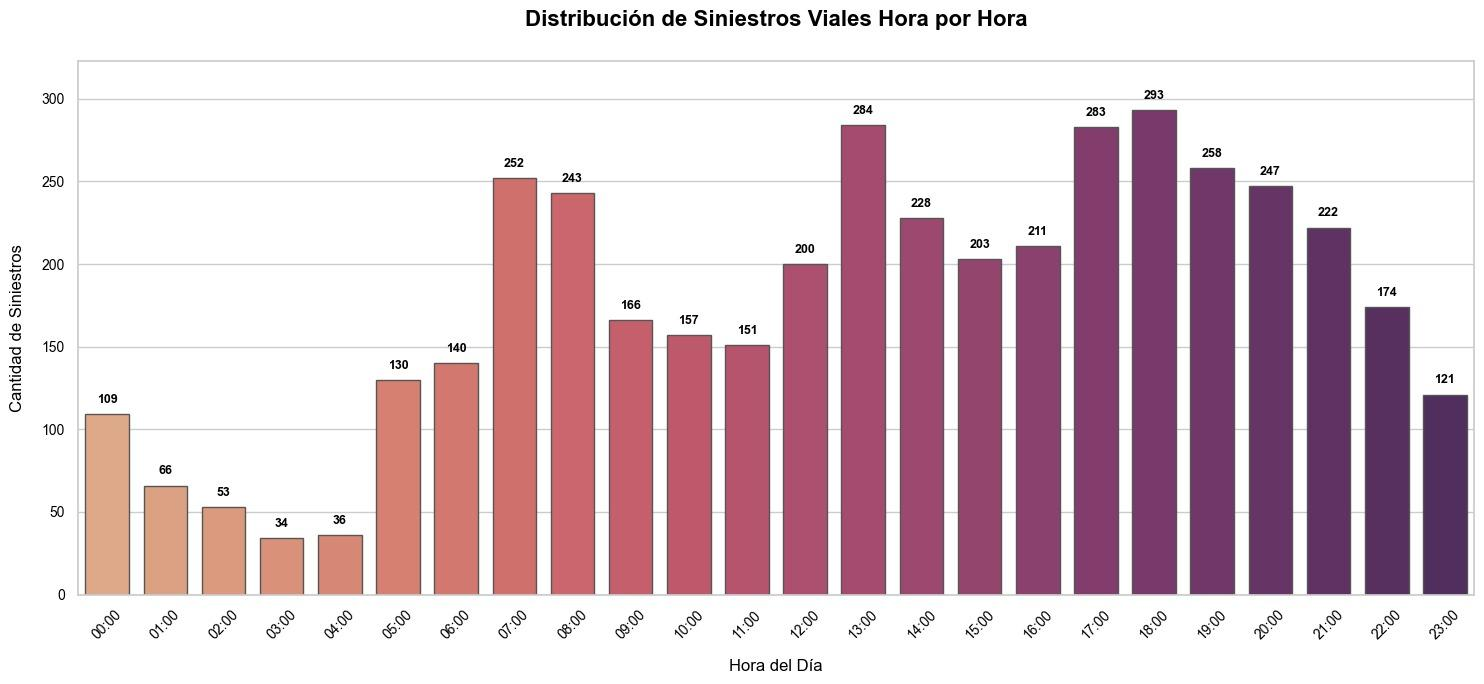
\includegraphics[width=\linewidth]{imagenes/image23.jpg}
\caption{Distribución del total de accidentes por hora del día}
\label{fig:distribucion-del-total-de-accidentes-por}
\notaflot{\fuentepropia{}, a partir de los datos provistos por el Ministerio Público Fiscal.}
\end{figure}

Para poder aplicar un modelo \xgboost{} (\eng{Extreme Gradient Boosting}) se modifica la forma en que el conjunto de datos representa la información. El objetivo es que cada registro, ordenado cronológicamente, contenga información dividida en tres partes: datos del pasado, datos del presente y la cantidad de accidentes que hubo en ese contexto. Para ello se utiliza la técnica de ventanas deslizantes, que consiste en traer al presente información del pasado por medio de retardos (formulación autorregresiva supervisada) y sumarla a los datos del presente para generar el contexto que explica la cantidad de víctimas de ese momento. Por ejemplo, para un viernes por la tarde puede reconstruirse el promedio de víctimas de la última semana, las víctimas del viernes anterior o las de las últimas doce horas, entre múltiples combinaciones con esta y otras variables, como las climáticas. Siguiendo este método, para generar un registro basta con un algoritmo que se desplace pasos hacia atrás en el tiempo, agregue la información requerida y la inscriba en el registro actual.

De esta manera cambia por completo lo que representan los datos. Antes se tenía una serie de registros que ubican cada accidente de manera irregular, con información que caracteriza el hecho en sí; ahora se tiene un conjunto de datos que representa el estado de un sistema (el tránsito de la ciudad de Córdoba) definido por una serie de características que, al variar en el tiempo, generan incrementos o decrementos del riesgo de accidente vial. Una vez entrenado, el modelo aprende a detectar los patrones que generan una subida en la cantidad de víctimas, así como qué combinación de variables hace que el riesgo permanezca bajo.

\subsection{Definición de la estructura de Ventanas Deslizantes}\label{definiciuxf3n-de-la-estructura-de-ventanas-deslizantes}

En este punto se define la variable objetivo del entrenamiento, es decir, la que el modelo intenta predecir a partir de las demás características del conjunto de datos. Se definió una variable denominada \var{TARGET\_CRITICO}, de naturaleza binaria, que toma el valor 1 cuando existe al menos una víctima de accidente vial y 0 cuando no hay víctimas. Esta variable es la que permite calcular los retardos que se mencionan más adelante.

Por otro lado se tienen las variables relacionadas con la dimensión del tiempo. El día está codificado con un 1 para el lunes, un 2 para el martes y así sucesivamente; análogamente se categorizan las franjas horarias (el 1 corresponde a la franja de 00:00 a 06:00 y el 2 al bloque contiguo) y el mes del año. En estas variables puede surgir un problema según el modelo que se utilice: el algoritmo no entiende que el tiempo es cíclico, de modo que para él el lunes está a una distancia de seis respecto del domingo, cuando en realidad también los separa una distancia de uno. Para resolverlo puede aplicarse una transformación seno-coseno a cada una de estas variables. En el caso de los árboles de decisión su uso no es del todo necesario, pero conviene aclararlo por si en el futuro se decide usar modelos complementarios como el perceptrón multicapa.

\begin{figure}[htbp]
\centering
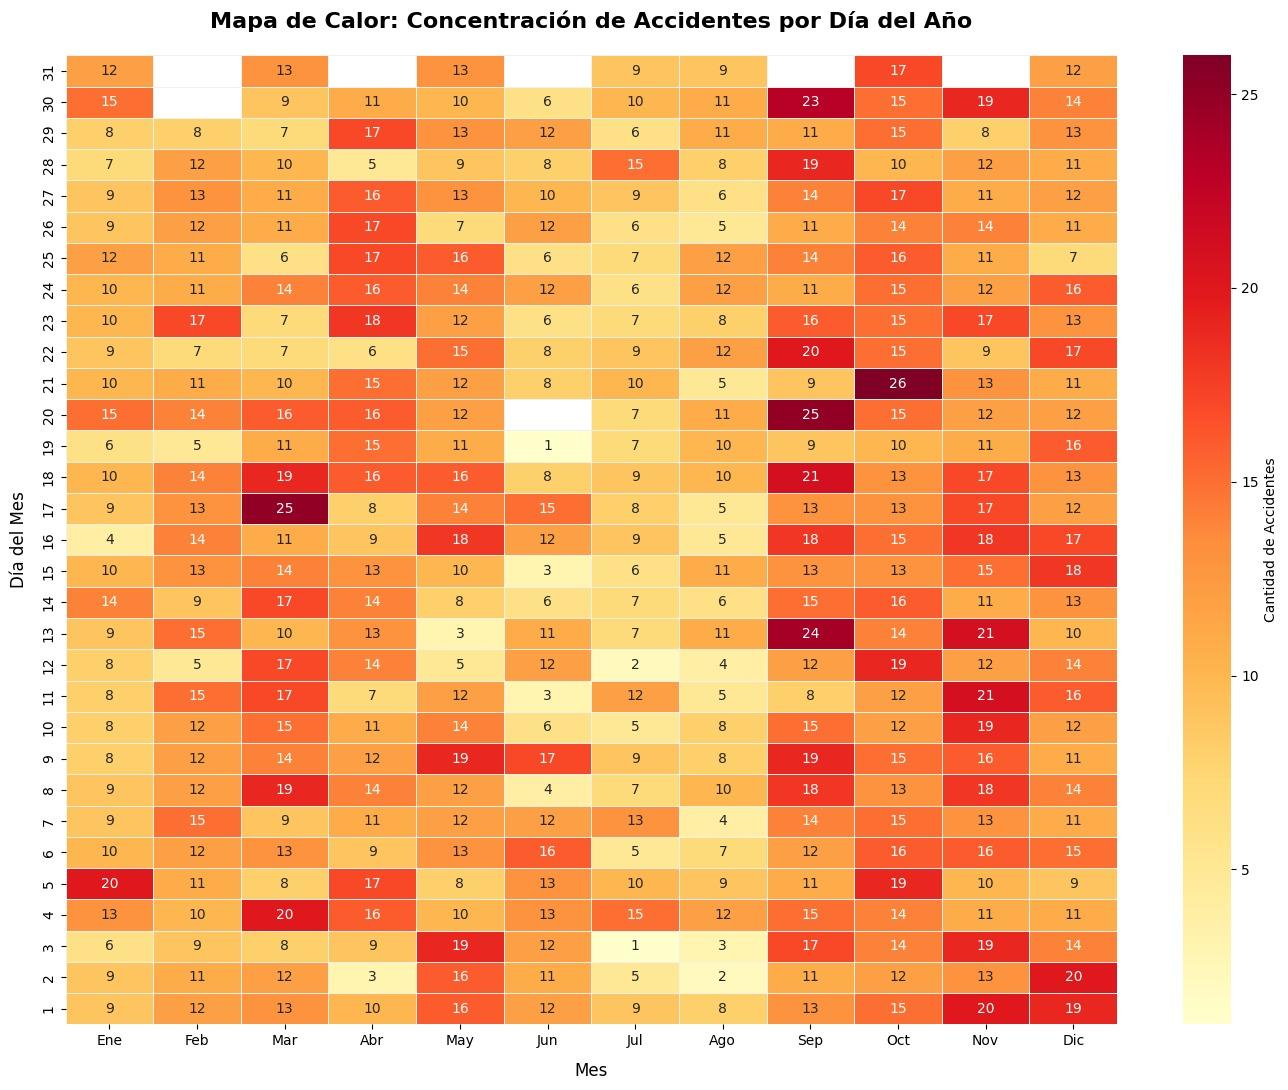
\includegraphics[width=\linewidth]{imagenes/image24.jpg}
\caption{Concentración de accidentes por día del año}
\label{fig:mapa-calor-dia-anio}
\notaflot{\fuentepropia{}.}
\end{figure}

Si se tiene presente la estrategia de las ventanas deslizantes, es razonable plantearse que una agregación de las víctimas de las horas pasadas puede no ser suficiente para un pronóstico con cierto grado de precisión, y que conviene generar variables que indiquen tendencia o inercia, bajo la sospecha de que una tendencia al alza en el corto plazo anticipa más accidentes en el futuro próximo. Es el caso de la variable \var{tendencia\_corto\_victimas}, que representa la diferencia entre las víctimas de las últimas seis horas y las de las últimas veinticuatro horas; el mismo principio se extiende a las variables de clima, de cantidad de lesionados y demás. La \cref{tab:estructura-y-tipos-de-datos-del-conjunto} detalla la configuración final del conjunto de datos.

\begin{longtable}[]{@{}rll@{}}
\caption{Estructura y tipos de datos del conjunto de entrenamiento}
\label{tab:estructura-y-tipos-de-datos-del-conjunto}\\
\toprule\noalign{}
\textbf{\#} & \textbf{Variable} & \textbf{Tipo de dato} \\
\midrule\noalign{}
\endfirsthead
\toprule\noalign{}
\textbf{\#} & \textbf{Variable} & \textbf{Tipo de dato} \\
\midrule\noalign{}
\endhead
\bottomrule\noalign{}
\endlastfoot
0 & \var{hora\_sin} & float64 \\
1 & \var{hora\_cos} & float64 \\
2 & \var{dia\_sin} & float64 \\
3 & \var{dia\_cos} & float64 \\
4 & \var{mes\_sin} & float64 \\
5 & \var{mes\_cos} & float64 \\
6 & \var{es\_fin\_de\_semana} & float64 \\
7 & tavg & float64 \\
8 & pres & float64 \\
9 & \var{cambio\_presion} & float64 \\
10 & \var{cambio\_temperatura} & float64 \\
11 & \var{victimas\_lag\_1} & float64 \\
12 & \var{lesiones\_lag\_1} & float64 \\
13 & \var{victimas\_lag\_4} & float64 \\
14 & \var{promedio\_victimas\_24h} & float64 \\
15 & \var{tendencia\_corto\_victimas} & float64 \\
16 & \var{aceleracion\_riesgo} & float64 \\
17 & \var{victimas\_mismo\_momento\_6d} & float64 \\
18 & \var{lesiones\_mismo\_momento\_6d} & float64 \\
19 & \var{tipomesESCOLAR\_2} & float64 \\
20 & \var{TARGET\_CRITICO} & int64 \\
\end{longtable}

\notaflot{El conjunto de datos consta de 2784 entradas (índice 0 a 2783) con un total de 21 variables, de las cuales 20 son de tipo continuo (float64) y 1 entera (int64).}

Si bien se detalla el resultado final, las variables no fueron seleccionadas arbitrariamente. La ingeniería de variables es, junto con el tratamiento inicial de los datos crudos, una de las etapas más extensas en tiempo y recursos de cualquier pipeline de aprendizaje automático, y este proyecto no fue la excepción: la configuración descripta surge de entrenar varios modelos, analizar sus métricas, ventajas y desventajas, y converger en el conjunto que se presenta.

\subsection{Entrenamiento del modelo XGBoost}\label{entrenamiento-del-modelo-xg-boosting}

Como se mencionó, la variable objetivo es binaria: vale uno cuando hay al menos una víctima de accidente vial y cero cuando no las hay. La estrategia seleccionada consiste en configurar el modelo como un regresor de Poisson, lo que no es un detalle menor, dado que también sería posible un clasificador binario que prediga directamente 0 o 1 (este experimento se realizó y no obtuvo un buen desempeño). Un regresor de Poisson tiene como salida un valor continuo que representa la tasa o expectativa de que ocurra al menos un accidente.

Para encontrar los mejores hiperparámetros (configuraciones previas al entrenamiento que influyen en la capacidad de generalización del modelo) se utilizó la búsqueda por grilla, que consiste en realizar varios entrenamientos con distintas configuraciones y retener la de mejores resultados. La \cref{tab:hiperparametros-optimizados-del-modelo} resume los valores seleccionados.

\begin{longtable}[]{@{}
>{\raggedright\arraybackslash}p{(\linewidth - 2\tabcolsep) * \real{0.3340}}
  >{\centering\arraybackslash}p{(\linewidth - 2\tabcolsep) * \real{0.3340}}@{}}
\caption{Hiperparámetros optimizados del modelo}
\label{tab:hiperparametros-optimizados-del-modelo}\\
\toprule\noalign{}
\textbf{Hiperparámetro} & \textbf{Valor} \\
\midrule\noalign{}
\endfirsthead
\toprule\noalign{}
\textbf{Hiperparámetro} & \textbf{Valor} \\
\midrule\noalign{}
\endhead
\bottomrule\noalign{}
\endlastfoot
colsample\_bytree & 0,9 \\
\var{learning\_rate} & 0,01 \\
\var{max\_depth} & 4 \\
\var{n\_estimators} & 100 \\
subsample & 0,7 \\
\end{longtable}

\notaflot{Hiperparámetros seleccionados mediante búsqueda y validación.}

Uno de los hiperparámetros más importantes en los modelos basados en árboles es \var{max\_depth}, la profundidad máxima que puede alcanzar un árbol. Una profundidad excesiva aumenta el riesgo de sobreajuste: el modelo se adapta demasiado a los datos de entrenamiento, captura incluso su ruido y pierde capacidad de generalización. Otro hiperparámetro relevante es \var{n\_estimators}, la cantidad de árboles que conforman el modelo. Un mayor número de estimadores puede mejorar la capacidad predictiva, al permitir que el modelo corrija progresivamente los errores de los árboles anteriores, pero un valor excesivo incrementa el tiempo de entrenamiento y, si no se regula mediante otros hiperparámetros como \var{learning\_rate}, aumenta también el riesgo de sobreajuste.

\begin{longtable}[]{@{}
>{\raggedright\arraybackslash}p{(\linewidth - 4\tabcolsep) * \real{0.3333}}
  >{\centering\arraybackslash}p{(\linewidth - 4\tabcolsep) * \real{0.3333}}
  >{\raggedright\arraybackslash}p{(\linewidth - 4\tabcolsep) * \real{0.3333}}@{}}
\caption{Métricas de error del modelo de línea base en el conjunto de prueba}
\label{tab:metricas-error-baseline}\\
\toprule\noalign{}
\textbf{Métrica de error} & \textbf{Valor} & \textbf{Interpretación} \\
\midrule\noalign{}
\endfirsthead
\toprule\noalign{}
\textbf{Métrica de error} & \textbf{Valor} & \textbf{Interpretación} \\
\midrule\noalign{}
\endhead
\bottomrule\noalign{}
\endlastfoot
Devianza de Poisson & 0,4662 & Medida de ajuste para datos de conteo (valores menores indican mejor ajuste). \\
MSE (Error Cuadrático Medio) & 0,1931 & Promedio de los errores cuadráticos entre el valor real y el predicho. \\
RMSE (Raíz del Error Cuadrático Medio) & 0,4394 & Error típico sobre la probabilidad estimada de que haya al menos una víctima. \\
\end{longtable}

\notaflot{Métricas calculadas sobre el conjunto de prueba independientemente del umbral de clasificación.}

Las métricas de la \cref{tab:metricas-error-baseline} permiten evaluar el desempeño del modelo desde distintas perspectivas, aunque ninguna por sí sola es suficiente. La devianza de Poisson cuantifica la discrepancia entre los valores observados y los estimados considerando la naturaleza discreta de la variable objetivo. El MSE, de 0,1931, penaliza en mayor medida las predicciones con desviaciones significativas, lo que lo vuelve útil para identificar errores de gran magnitud. A partir de él se obtiene el RMSE, de 0,4394.

Estas métricas no tienen un valor de referencia absoluto y deben interpretarse en comparación con un modelo trivial. Una predicción constante igual a la proporción de bloques críticos (0,711) obtiene un error cuadrático de 0,2055, mientras que el modelo obtiene 0,1931, una mejora del \qty{6}{\percent}. El modelo, por lo tanto, extrae información útil de los datos, aunque en una magnitud acotada.

\subsection{Evaluación y predicción}\label{evaluaciuxf3n-y-predicciuxf3n}

Para integrar este modelo en el sistema de alerta temprana se toman sus salidas continuas y se agrega una capa de decisión que determina si emitir o no la alerta. Para ello se define un umbral (\eng{threshold}): si la salida del modelo lo supera se activa la alarma y, en caso contrario, no. El problema pasa a ser definir el umbral más conveniente; para ello se analizaron múltiples alternativas y se seleccionó la que minimiza el error en el conjunto de validación. La \cref{tab:configuracion-del-umbral-del-sistema-de-} presenta el valor adoptado y la \cref{tab:matriz-de-confusion-del-modelo-de-clasif}, la matriz de confusión resultante.

\begin{longtable}[]{@{}
>{\raggedright\arraybackslash}p{(\linewidth - 4\tabcolsep) * \real{0.3333}}
  >{\centering\arraybackslash}p{(\linewidth - 4\tabcolsep) * \real{0.3333}}
  >{\raggedright\arraybackslash}p{(\linewidth - 4\tabcolsep) * \real{0.3333}}@{}}
\caption{Configuración del umbral del sistema de alerta}
\label{tab:configuracion-del-umbral-del-sistema-de-}\\
\toprule\noalign{}
\textbf{Parámetro} & \textbf{Valor} & \textbf{Descripción} \\
\midrule\noalign{}
\endfirsthead
\toprule\noalign{}
\textbf{Parámetro} & \textbf{Valor} & \textbf{Descripción} \\
\midrule\noalign{}
\endhead
\bottomrule\noalign{}
\endlastfoot
Umbral de alerta & 0,65 & Si la salida predicha supera este valor, la salida del sistema es 1 (alarma activada). \\
\end{longtable}

\notaflot{El valor de umbral define la transición del estado normal al estado de alerta crítica. Un valor demasiado bajo activa la alarma permanentemente, satura al usuario y logra el efecto contrario al buscado. Además, el umbral puede modificarse en el producto final sin reentrenar el modelo.}

\begin{table}[htbp]
\centering
\caption{Matriz de confusión del modelo de línea base}
\label{tab:matriz-de-confusion-del-modelo-de-clasif}
\small
\begin{tabular}{@{}lccc@{}}
\toprule
& \multicolumn{2}{c}{\textbf{Predicho}} & \\
\cmidrule(lr){2-3}
\textbf{Estado real} & \textbf{Normal (0)} & \textbf{Crítico (1)} & \textbf{Total real} \\
\midrule
Normal (0) & 62 & 99 & 161 \\
Crítico (1) & 50 & 346 & 396 \\
\midrule
\textbf{Total predicho} & \textbf{112} & \textbf{445} & \textbf{557} \\
\bottomrule
\end{tabular}
\notaflot{Muestras evaluadas sobre el conjunto de prueba ($N = 557$). La clase crítica corresponde a situaciones con víctimas esperadas (salida $= 1$). \fuentepropia{}.}
\end{table}

\subsection{Análisis de los resultados de modelo Baseline}\label{anuxe1lisis-de-los-resultados-de-modelo-baseline}\label{analisis-resultados-baseline}

Como el modelo está construido sobre árboles de decisión, es posible extraer la importancia de las variables, lo que permite garantizar la explicabilidad, en línea con la norma ISO/IEC 42001. La \cref{fig:contribucion-de-cada-variable-a-la-capac} resume esos resultados.

\begin{figure}[htbp]
\centering
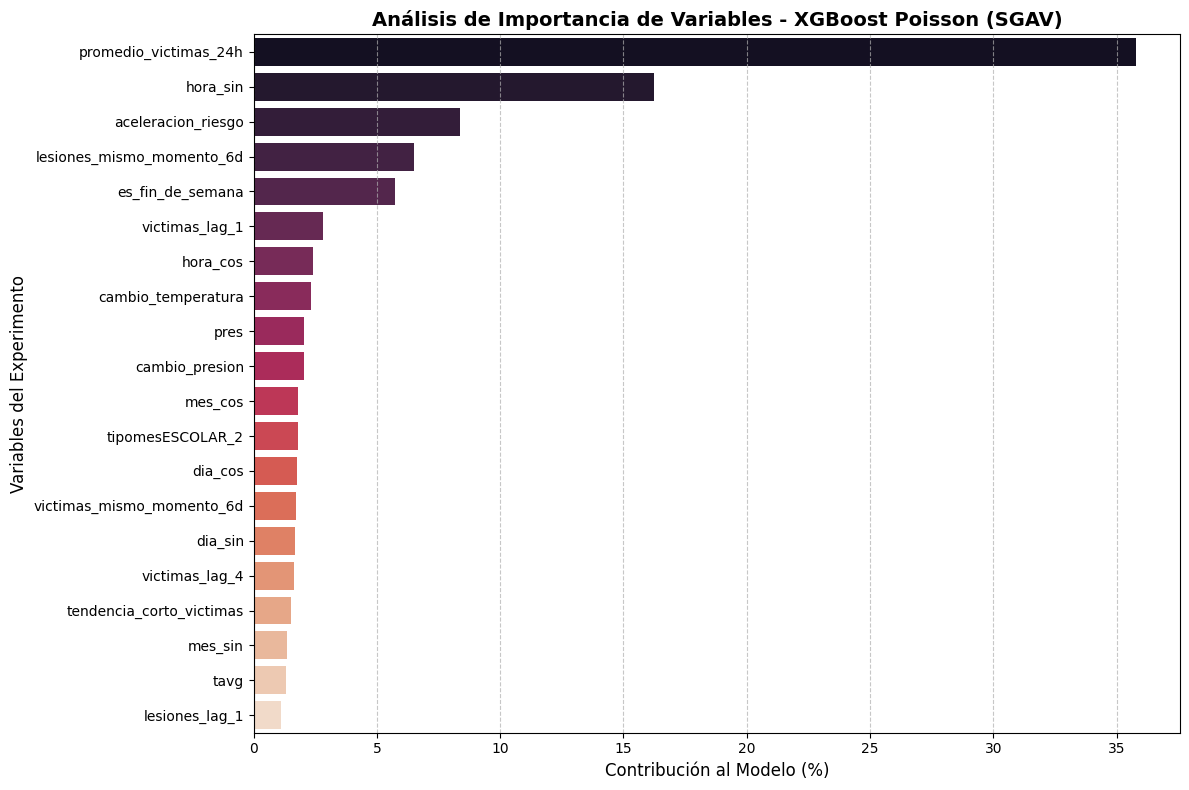
\includegraphics[width=\linewidth]{imagenes/image12.png}
\caption{Contribución de cada variable a la capacidad de predicción del modelo}
\label{fig:contribucion-de-cada-variable-a-la-capac}
\notaflot{\fuentepropia{}, según la salida del modelo entrenado.}
\end{figure}

Los resultados indican que el promedio de víctimas de las últimas 24 horas tiene la mayor contribución a la predicción, del orden del \qty{35}{\percent}, seguido por la componente seno del bloque horario, con un \qty{15}{\percent}. El pasado cercano y el bloque horario explican entonces poco más de la mitad de la predicción. Puede afirmarse que el riesgo de que existan accidentes depende mayoritariamente de cómo vienen evolucionando las víctimas en el pasado cercano: las primeras seis variables concentran el \qty{80}{\percent} de la contribución, y de ellas cuatro se refieren a lo ocurrido y solo dos al presente, la franja horaria (\var{hora\_sin}) y el fin de semana (\var{es\_fin\_de\_semana}).

También se observa que variables que se pensaba que podían influir notablemente, como las climatológicas (\var{cambio\_temperatura}, \var{pres}, \var{cambio\_presion}, \var{tavg}), aportan poco a la capacidad de predicción. Esta información es especialmente importante para el producto final: si una variable resulta irrelevante, puede optarse por no incluirla y, en consecuencia, no tener que recolectarla, procesarla ni entregarla al modelo.

\begin{longtable}[]{@{}
>{\raggedright\arraybackslash}p{(\linewidth - 6\tabcolsep) * \real{0.2500}}
  >{\centering\arraybackslash}p{(\linewidth - 6\tabcolsep) * \real{0.2500}}
  >{\centering\arraybackslash}p{(\linewidth - 6\tabcolsep) * \real{0.2500}}
  >{\raggedright\arraybackslash}p{(\linewidth - 6\tabcolsep) * \real{0.2500}}@{}}
\caption{Métricas del modelo para la clase crítica (1) y métricas globales}
\label{tab:metricas-del-modelo-de-clasificacion-par}\\
\toprule\noalign{}
\textbf{Métrica} & \textbf{Porcentaje} & \textbf{Valor decimal} & \textbf{Interpretación en el sistema} \\
\midrule\noalign{}
\endfirsthead
\toprule\noalign{}
\textbf{Métrica} & \textbf{Porcentaje} & \textbf{Valor decimal} & \textbf{Interpretación en el sistema} \\
\midrule\noalign{}
\endhead
\bottomrule\noalign{}
\endlastfoot
Exactitud global & \qty{73.2}{\percent} & 0,73 & Porcentaje global de predicciones correctas sobre el total de casos. \\
Sensibilidad en crítico & \qty{87.4}{\percent} & 0,87 & Porcentaje de eventos críticos capturados. \\
Precisión en crítico & \qty{77.8}{\percent} & 0,78 & Porcentaje de alertas emitidas que resultaron ser eventos críticos. \\
F1 en crítico & \qty{82.3}{\percent} & 0,82 & Media armónica entre la precisión y la sensibilidad para la clase crítica. \\
\end{longtable}

\notaflot{Las métricas evalúan el desempeño focalizado en la detección oportuna de eventos de riesgo.}

A partir de la matriz de confusión de la \cref{tab:matriz-de-confusion-del-modelo-de-clasif} se calculan las métricas de la \cref{tab:metricas-del-modelo-de-clasificacion-par}. La exactitud representa el porcentaje de predicciones correctas (408) sobre los 557 casos de prueba, es decir, el \qty{73.2}{\percent}. Como se intenta predecir un evento crítico, para los usuarios del producto interesa evaluar el desempeño específico sobre él.

La sensibilidad representa el porcentaje de eventos críticos reales que capturó el modelo: el \qty{87.4}{\percent} (346 de 396 casos). La precisión la complementa: representa el porcentaje de alertas emitidas que efectivamente correspondieron a bloques con víctimas. Es un punto de especial relevancia, porque la precisión es lo que el usuario percibe directamente: si de 445 alarmas 346 corresponden a bloques con víctimas, esa proporción incidirá en cómo percibe el riesgo cada vez que ve una alerta. Si el modelo detectara el \qty{100}{\percent} de los accidentes emitiendo alertas constantemente, la precisión caería y el usuario terminaría fatigándose y bajando la guardia.

La exactitud (\qty{73.2}{\percent}) y la sensibilidad en la clase crítica (\qty{87.4}{\percent}) deben leerse frente a la regla de alerta permanente, que obtiene \qty{71.1}{\percent} y \qty{100}{\percent} respectivamente (\cref{tab:res-baseline-referencia}). En la clase crítica, el modelo no supera a esa regla: su aporte se concentra en la clase normal, donde identifica el \qty{38.5}{\percent} de los bloques sin víctimas, mientras que la regla trivial no identifica ninguno.

El F1 es la media armónica entre la precisión y la sensibilidad, por lo que solo alcanza valores elevados cuando ambas son buenas simultáneamente. A diferencia de la exactitud, ofrece una evaluación más representativa de la capacidad del modelo para identificar la clase de interés. En este caso, el F1 de la clase crítica (al menos una víctima) alcanzó un \qty{82.3}{\percent}.

\begin{longtable}[]{@{}
>{\raggedright\arraybackslash}p{(\linewidth - 4\tabcolsep) * \real{0.3333}}
  >{\centering\arraybackslash}p{(\linewidth - 4\tabcolsep) * \real{0.3333}}
  >{\raggedright\arraybackslash}p{(\linewidth - 4\tabcolsep) * \real{0.3333}}@{}}
\caption{Desempeño y errores del modelo en la clase normal (0)}
\label{tab:desempeno-y-errores-del-modelo-en-la-cla}\\
\toprule\noalign{}
\textbf{Métrica / Concepto} & \textbf{Valor} & \textbf{Interpretación en el sistema} \\
\midrule\noalign{}
\endfirsthead
\toprule\noalign{}
\textbf{Métrica / Concepto} & \textbf{Valor} & \textbf{Interpretación en el sistema} \\
\midrule\noalign{}
\endhead
\bottomrule\noalign{}
\endlastfoot
Sensibilidad en normal & \qty{38.5}{\percent} & Proporción de momentos seguros reales identificados. \\
Falsas alertas (falsos positivos) & 99 & Situaciones sin víctimas en las que el sistema emitió erróneamente una alerta. \\
Críticos no detectados (falsos negativos) & 50 & Situaciones con víctimas en las que el sistema no activó la alerta. \\
\end{longtable}
\notaflot{\fuentepropia{} a partir de la \cref{tab:matriz-de-confusion-del-modelo-de-clasif}.}

Aquí se advierte la dificultad fundamental de predecir eventos como los siniestros viales. En la clase normal (momentos sin víctimas) la sensibilidad es del \qty{38.5}{\percent}, producto de identificar correctamente 62 de 161 momentos seguros. Además se registran 99 falsos positivos y 50 momentos sin alerta en los que hubo víctimas. Estos resultados sugieren que el sistema todavía no discrimina con gran capacidad entre momentos seguros y momentos riesgosos.

El \xgboost{} descripto no es un modelo para llevar a producción tal como está, lo que no significa que no sirva: los modelos de línea base son fundamentales en el desarrollo de productos basados en inteligencia artificial. Este en particular sirve como referencia para comparar los modelos que se entrenen en el futuro, para identificar las variables que más contribuyen a la capacidad predictiva, para definir qué métricas observar y para seleccionar hiperparámetros, además de fijar la forma en que se agregan los datos, que es determinante no solo para el modelo sino también para los requerimientos del producto final.

\section{Gestión del proyecto}\label{gestiuxf3n-del-proyecto}

Esta sección reúne los aspectos de gestión del proyecto que acompañan al producto: las dependencias de las que depende su funcionamiento, la gestión de riesgos y la evaluación de impacto según las normas ISO/IEC 42001 e ISO/IEC 23894, y el flujograma que integra el proceso de extremo a extremo.

\subsection{Dependencias tecnológicas y funcionales}\label{dependencias-tecnoluxf3gicas-y-funcionales}

Las dependencias tecnológicas y funcionales aplicables a un proyecto de software basado en inteligencia artificial pueden ser sumamente extensas dependiendo de la complejidad del sistema, dado que en este caso se analiza un MVP se tendrán en cuenta sólo las aplicables al alcance de una prueba de concepto de estas características.

Primeramente se deben analizar las dependencias funcionales, es decir, todas las condiciones del negocio o los procesos operativos en los cuales la intervención humana es necesaria para que el producto o sistema funcione. Se tiene por ejemplo el caso de la carga de datos, una falla en este proceso es vital para el sistema, si la información no se carga a tiempo o se introducen datos erróneos el resultado puede ser de impacto crítico en el caso de lo primero (el sistema queda inutilizable) o de impacto medio en el segundo caso (el sistema funciona pero con precisión reducida).

Por otra parte se tienen las dependencias tecnológicas, que son los componentes de hardware, software, servicios en la nube, APIs o bases de datos de los que depende la solución para recopilar datos, entrenar modelos o mostrar resultados. Con el mismo criterio mencionado anteriormente se destaca el Centro de Cómputos de Alto Desempeño, tanto en su servidor donde se aloja el servicio web como sus clusters de cómputo como Serafin o Mendieta donde se entrenan los modelos. El servidor de CCAD donde se aloja el servicio genera una dependencia crítica porque sin él es imposible alertar a los usuarios del MPF, en cambio, los clusters donde se entrenan los modelos no generan un impacto que comprometa al sistema dado que no es necesario reentrenar constantemente para mantener la precisión. Por último se encuentra una dependencia referida al consumo de APIs meteorológicas para la extracción de datos climáticos necesarios para realizar las predicciones, si bien es posible configurar el sistema para que tenga APIs como segunda opción (si la principal se cae), el impacto es bajo ya que no tener esta información disponible no reduce de manera significativa el desempeño del modelo.

\begin{longtable}[]{@{}
>{\raggedright\arraybackslash}p{(\linewidth - 4\tabcolsep) * \real{0.2281}}
  >{\raggedright\arraybackslash}p{(\linewidth - 4\tabcolsep) * \real{0.1927}}
  >{\raggedright\arraybackslash}p{(\linewidth - 4\tabcolsep) * \real{0.5428}}@{}}
\caption{Matriz de dependencias}
\label{tab:matriz-de-dependencias}\\
\toprule\noalign{}
\textbf{Dependencia} & \textbf{Tipo} & \textbf{Impacto} \\
\midrule\noalign{}
\endfirsthead
\toprule\noalign{}
\textbf{Dependencia} & \textbf{Tipo} & \textbf{Impacto} \\
\midrule\noalign{}
\endhead
\bottomrule\noalign{}
\endlastfoot
Carga de Datos & Funcional & Crítica: Se pierde la secuencialidad del modelo \\
Clasificación de la lesión & Funcional & Media: El modelo pierde precisión \\
CCAD Servidor & Tecnológica & Crítica: El modelo no está disponible \\
CCAD Serafin & Tecnológica & Baja: Impide el reentrenamiento del modelo \\
API Meteo & Tecnológica & Baja: El modelo no pierde precisión de manera significativa \\
\end{longtable}

\notaflot{\fuentepropia{}.}

\subsection{Gestión de riesgos}\label{gestiuxf3n-de-riesgos}\label{gestion-de-riesgos}

La gestión de riesgos del sistema de Alerta Temprana de Accidentes Viales se estructuró siguiendo los lineamientos de la cláusula 6.1 de la norma ISO/IEC 42001:2023 a nivel general y por otro lado a la orientación metodológica de la norma ISO/IEC 23894:2023. La primera establece qué debe producir el proceso en términos de criterios definidos, una evaluación con resultados comparables, un plan de tratamiento y una evaluación de impacto. Mientras que la segunda aporta el procedimiento y, en particular, el relevamiento de fuentes de riesgo de su Anexo B, empleado en este documento como marco de identificación.

Es necesario distinguir dos ejercicios que la norma 42001 requiere por separado y que con frecuencia se confunden. La cláusula 6.1.2 refiere a la evaluación de los riesgos que afectan a los objetivos de la organización, mientras que la cláusula 6.1.4 refiere a la evaluación del impacto del sistema sobre individuos, grupos y sociedad. El presente apartado desarrolla el primero; el segundo se trata en el apartado siguiente. La relación entre ambos es de alimentación: los impactos identificados sobre terceros se incorporan al registro de riesgos en la medida en que generan exposición institucional, legal o reputacional para los organismos involucrados.

El alcance de esta evaluación comprende el ciclo completo del dato y de la predicción bajo el esquema de trabajo que se definió previamente a lo largo de este documento, que es de responsabilidad compartida: el Ministerio Público Fiscal es el origen de los datos y el destinatario de las alertas, mientras que el Laboratorio de Investigación y Desarrollo de Software e Inteligencia Artificial concentra el procesamiento, el entrenamiento y la generación de las predicciones. Al no delegar completamente la operación del sistema en su conjunto, se generan dos superficies de riesgo propias y se tratan como tales, el ingreso de datos y la emisión de alertas.

\subsection{Criterios de Riesgo}\label{criterios-de-riesgo}

Con el fin de que la evaluación produzca resultados comparables entre sí, se definieron escalas cualitativas de cuatro niveles para la probabilidad de ocurrencia y para la severidad del impacto. Se optó por cuatro niveles en lugar de los tres habituales para discriminar mejor los riesgos intermedios. El nivel de riesgo resultante se obtiene del producto de ambos valores.

\begin{longtable}[]{@{}
>{\raggedright\arraybackslash}p{(\linewidth - 4\tabcolsep) * \real{0.1606}}
  >{\centering\arraybackslash}p{(\linewidth - 4\tabcolsep) * \real{0.0964}}
  >{\raggedright\arraybackslash}p{(\linewidth - 4\tabcolsep) * \real{0.7066}}@{}}
\caption{Escala de probabilidad de ocurrencia}
\label{tab:escala-de-probabilidad-de-ocurrencia}\\
\toprule\noalign{}
\textbf{Nivel} & \textbf{Valor} & \textbf{Criterio de asignación} \\
\midrule\noalign{}
\endfirsthead
\toprule\noalign{}
\textbf{Nivel} & \textbf{Valor} & \textbf{Criterio de asignación} \\
\midrule\noalign{}
\endhead
\bottomrule\noalign{}
\endlastfoot
Baja & 1 & No se ha observado durante el desarrollo y no existen indicios de que pueda materializarse en el horizonte del prototipo. \\
Media & 2 & Es plausible; existen condiciones que podrían habilitarla, aunque no se ha manifestado. \\
Alta & 3 & Se ha manifestado de forma ocasional durante el desarrollo o es esperable en condiciones normales de operación. \\
Muy alta & 4 & Se verifica de manera sistemática en la situación actual del proyecto. \\
\end{longtable}

\notaflot{\fuentepropia{} sobre la base de ISO/IEC 23894:2023.}

\begin{longtable}[]{@{}
>{\raggedright\arraybackslash}p{(\linewidth - 4\tabcolsep) * \real{0.1606}}
  >{\centering\arraybackslash}p{(\linewidth - 4\tabcolsep) * \real{0.0964}}
  >{\raggedright\arraybackslash}p{(\linewidth - 4\tabcolsep) * \real{0.7066}}@{}}
\caption{Escala de severidad del impacto}
\label{tab:escala-de-severidad-del-impacto}\\
\toprule\noalign{}
\textbf{Nivel} & \textbf{Valor} & \textbf{Criterio de asignación} \\
\midrule\noalign{}
\endfirsthead
\toprule\noalign{}
\textbf{Nivel} & \textbf{Valor} & \textbf{Criterio de asignación} \\
\midrule\noalign{}
\endhead
\bottomrule\noalign{}
\endlastfoot
Menor & 1 & Afecta la comodidad del desarrollo sin comprometer resultados ni usuarios. \\
Moderado & 2 & Degrada el desempeño del sistema o retrasa el cronograma, sin invalidar los resultados obtenidos. \\
Mayor & 3 & Invalida resultados, inutiliza temporalmente el sistema o afecta la confianza del usuario final en la herramienta. \\
Crítico & 4 & Compromete derechos de terceros, obligaciones legales del organismo o la viabilidad del proyecto. \\
\end{longtable}

\notaflot{\fuentepropia{} sobre la base de ISO/IEC 23894:2023.}

\begin{longtable}[]{@{}
>{\raggedright\arraybackslash}p{(\linewidth - 8\tabcolsep) * \real{0.1931}}
  >{\centering\arraybackslash}p{(\linewidth - 8\tabcolsep) * \real{0.1931}}
  >{\centering\arraybackslash}p{(\linewidth - 8\tabcolsep) * \real{0.1931}}
  >{\centering\arraybackslash}p{(\linewidth - 8\tabcolsep) * \real{0.1931}}
  >{\centering\arraybackslash}p{(\linewidth - 8\tabcolsep) * \real{0.1931}}@{}}
\caption{Matriz de nivel de riesgo}
\label{tab:matriz-de-nivel-de-riesgo}\\
\toprule\noalign{}
\textbf{Probabilidad / Impacto} & \textbf{Menor (1)} & \textbf{Moderado (2)} & \textbf{Mayor (3)} & \textbf{Crítico (4)} \\
\midrule\noalign{}
\endfirsthead
\toprule\noalign{}
\textbf{Probabilidad / Impacto} & \textbf{Menor (1)} & \textbf{Moderado (2)} & \textbf{Mayor (3)} & \textbf{Crítico (4)} \\
\midrule\noalign{}
\endhead
\bottomrule\noalign{}
\endlastfoot
Muy alta (4) & Amarillo (4) & Naranja (8) & Rojo (12) & Rojo (16) \\
Alta (3) & Verde (3) & Amarillo (6) & Naranja (9) & Rojo (12) \\
Media (2) & Verde (2) & Amarillo (4) & Amarillo (6) & Naranja (8) \\
Baja (1) & Verde (1) & Verde (2) & Verde (3) & Amarillo (4) \\
\end{longtable}

\notaflot{\fuentepropia{}. El valor entre paréntesis corresponde al producto de la probabilidad por el impacto.}

Respecto del nivel de riesgo declarado para la etapa actual se define en función del nivel de madurez tecnológica. Al tratarse de un prototipo en TRL 3 que no se encuentra desplegado en operación real y que no sustituye ningún procedimiento vigente del organismo, se aceptan sin acción los riesgos de nivel verde y amarillo. Los riesgos de nivel naranja se documentan con un tratamiento previsto que puede posponerse a etapas de mayor madurez. Los riesgos de nivel rojo requieren tratamiento explícito o, en su defecto, una declaración de aceptación fundamentada, y constituyen condición de salida hacia niveles TRL superiores.

\subsection{Identificación y Valoración de Riesgos}\label{identificaciuxf3n-y-valoraciuxf3n-de-riesgos}\label{identificacion-y-valoracion-de-riesgos}

La identificación se realizó recorriendo el catálogo de fuentes de riesgo del Anexo B de la norma ISO/IEC 23894:2023 y contrastando cada categoría contra las características concretas del sistema desarrollado. El relevamiento incorpora además las dependencias funcionales y tecnológicas documentadas en el apartado anterior, que constituyen la base de los riesgos R8 y R9. El resultado se presenta en la \cref{tab:registro-de-identificacion-y-valoracion-}.

\begin{longtable}[]{@{}
>{\raggedright\arraybackslash}p{(\linewidth - 10\tabcolsep) * \real{0.0698}}
  >{\raggedright\arraybackslash}p{(\linewidth - 10\tabcolsep) * \real{0.3813}}
  >{\raggedright\arraybackslash}p{(\linewidth - 10\tabcolsep) * \real{0.2524}}
  >{\centering\arraybackslash}p{(\linewidth - 10\tabcolsep) * \real{0.0483}}
  >{\centering\arraybackslash}p{(\linewidth - 10\tabcolsep) * \real{0.0483}}
  >{\centering\arraybackslash}p{(\linewidth - 10\tabcolsep) * \real{0.1665}}@{}}
\caption{Registro de identificación y valoración de riesgos}
\label{tab:registro-de-identificacion-y-valoracion-}\\
\toprule\noalign{}
\textbf{ID} & \textbf{Descripción del riesgo} & \textbf{Fuente de riesgo (Anexo B, ISO/IEC 23894)} & \textbf{P} & \textbf{I} & \textbf{Nivel} \\
\midrule\noalign{}
\endfirsthead
\toprule\noalign{}
\textbf{ID} & \textbf{Descripción del riesgo} & \textbf{Fuente de riesgo (Anexo B, ISO/IEC 23894)} & \textbf{P} & \textbf{I} & \textbf{Nivel} \\
\midrule\noalign{}
\endhead
\bottomrule\noalign{}
\endlastfoot
R1 & Errores de transcripción y falta de normalización derivados de la carga manual de los siniestros por parte del personal administrativo. & Calidad y procedencia de los datos & 3 & 3 & Naranja (9) \\
R2 & Latencia entre la ocurrencia del siniestro y su digitalización, que altera la posición temporal del evento en la serie. & Calidad de los datos / Complejidad del entorno & 4 & 3 & Rojo (12) \\
R3 & Sesgo de subregistro: la base contiene únicamente siniestros con intervención judicial y no representa la siniestralidad total de la ciudad. & Sesgo algorítmico & 4 & 2 & Naranja (8) \\
R4 & Reidentificación de personas involucradas por cruce de fecha, franja horaria, georreferenciación y tipo de lesión, no verificada hasta la fecha. & Privacidad y protección de datos & 3 & 4 & Rojo (12) \\
R5 & Fatiga de alerta por exceso de falsos positivos, con la consiguiente pérdida de confianza del usuario en la herramienta. & Nivel de automatización / Uso del sistema & 3 & 3 & Naranja (9) \\
R6 & Sesgo de automatización: delegación del juicio profesional en la salida del sistema sin contraste con otras fuentes. & Nivel de automatización & 2 & 3 & Amarillo (6) \\
R7 & Ausencia de un procedimiento formalizado de supervisión humana para validar o desestimar las alertas antes de su uso. & Supervisión humana / Uso del sistema & 3 & 3 & Naranja (9) \\
R8 & Indisponibilidad del servidor del CCAD que aloja el servicio, con interrupción total de la emisión de alertas. & Hardware e infraestructura & 2 & 3 & Amarillo (6) \\
R9 & Interrupción del suministro de datos climáticos por caída de la API meteorológica. & Complejidad del entorno de despliegue & 2 & 2 & Amarillo (4) \\
R10 & Uso desviado del sistema hacia finalidades no previstas, riesgo latente que se activaría con la incorporación de predicción georreferenciada por zonas. & Uso previsto / Impacto social & 2 & 3 & Amarillo (6) \\
R11 & Dependencia de personas clave y ausencia de un esquema definido de continuidad o transferencia del sistema. & Ciclo de vida del sistema de IA & 3 & 2 & Amarillo (6) \\
\end{longtable}

\notaflot{\fuentepropia{}. P: probabilidad; I: impacto, valorados según las \cref{tab:escala-de-probabilidad-de-ocurrencia,tab:escala-de-severidad-del-impacto}. El nivel resulta de la \cref{tab:matriz-de-nivel-de-riesgo}. Las categorías de fuente corresponden al Anexo B de ISO/IEC 23894:2023. Los riesgos R8 y R9 se corresponden con las dependencias de impacto crítico y medio identificadas en la matriz de dependencias tecnológicas y funcionales.}

\subsection{Plan de Mitigación de Riesgos}\label{plan-de-mitigacion-de-riesgos}

La \cref{tab:plan-de-mitigacion-de-riesgos} consigna el tratamiento propuesto para cada riesgo identificado y el nivel residual estimado al cierre de la etapa actual. Se indica asimismo el actor responsable, considerando el esquema de responsabilidad compartida mencionado al inicio del apartado.

\begin{longtable}[]{@{}
>{\raggedright\arraybackslash}p{(\linewidth - 6\tabcolsep) * \real{0.0697}}
  >{\raggedright\arraybackslash}p{(\linewidth - 6\tabcolsep) * \real{0.4770}}
  >{\raggedright\arraybackslash}p{(\linewidth - 6\tabcolsep) * \real{0.1768}}
  >{\raggedright\arraybackslash}p{(\linewidth - 6\tabcolsep) * \real{0.2412}}@{}}
\caption{Plan de mitigación de riesgos}
\label{tab:plan-de-mitigacion-de-riesgos}\\
\toprule\noalign{}
\textbf{ID} & \textbf{Tratamiento propuesto} & \textbf{Responsable} & \textbf{Residual en TRL 3} \\
\midrule\noalign{}
\endfirsthead
\toprule\noalign{}
\textbf{ID} & \textbf{Tratamiento propuesto} & \textbf{Responsable} & \textbf{Residual en TRL 3} \\
\midrule\noalign{}
\endhead
\bottomrule\noalign{}
\endlastfoot
R1 & Reducir. Validaciones automáticas de rango y consistencia en la etapa de curado, y documentación del diccionario de datos acordada con el equipo de datos del MPF. & LIDeSIA / Equipo de datos del MPF & Amarillo. Aceptado. \\
R2 & Reducir. Incorporación de la fecha de digitalización como variable de control, evaluación del desfase medio y definición de una ventana de corte que excluya los bloques aún incompletos. & LIDeSIA / MPF & Naranja. Condición de salida hacia TRL 4. \\
R3 & Aceptar con declaración. La población objetivo del sistema son precisamente los eventos con intervención judicial, por lo que el sesgo resulta parcialmente alineado con el caso de uso. Se documenta como limitación de generalización. & LIDeSIA & Naranja. Aceptado con declaración. \\
R4 & Reducir. Verificación de unicidad de los registros por combinación de cuasi-identificadores y, en caso de detectarse casos únicos, agregación espacial o temporal previa a cualquier publicación o difusión del conjunto de datos. & LIDeSIA / MPF & Rojo. Tratamiento pendiente y condición de salida hacia TRL 4. \\
R5 & Reducir. Calibración del umbral de decisión priorizando la precisión por sobre la sensibilidad, con aceptación explícita de la consecuencia que ello implica sobre los eventos no detectados, conforme a la política declarada en el apartado siguiente. & LIDeSIA & Amarillo. Tratamiento en curso. \\
R6 & Reducir. Comunicación de la alerta acompañada de su intervalo de predicción y no como valor puntual, y declaración del carácter complementario del sistema respecto del procedimiento vigente, de modo que la incertidumbre resulte visible para el usuario. & LIDeSIA & Amarillo. Aceptado. \\
R7 & Reducir, de forma compartida y diferida. Definición de un procedimiento de validación humana previa a la actuación, con registro de la decisión adoptada, prevista para la etapa de integración con el MPF. & MPF / LIDeSIA & Naranja. Condición de salida hacia TRL 4. \\
R8 & Aceptar con tratamiento diferido. Definición del requisito de disponibilidad y del esquema de contingencia prevista para la etapa de despliegue. & CCAD / LIDeSIA & Amarillo. Aceptado. \\
R9 & Evitar. Dado que el análisis de importancia de variables del modelo de línea de base evidenció una contribución marginal de las variables climáticas, se evalúa su exclusión del conjunto de entradas, lo que elimina la fuente de riesgo. Como alternativa, configuración de una fuente meteorológica secundaria. & LIDeSIA & Verde, sujeto a la confirmación de la exclusión de la variable. \\
R10 & Evitar. Declaración explícita del uso previsto y de los usos no admitidos del sistema, incorporada al apartado de definición de requisitos, y nueva evaluación de impacto como condición previa a la incorporación de predicción georreferenciada. & LIDeSIA / MPF & Amarillo. Latente. \\
R11 & Reducir. Documentación del código y de los procedimientos en repositorio versionado, como condición previa a cualquier esquema de transferencia. & LIDeSIA & Amarillo. Aceptado. \\
\end{longtable}

\notaflot{\fuentepropia{}. Las opciones de tratamiento corresponden a las categorías de ISO 31000:2018 adoptadas por ISO/IEC 23894:2023: evitar la fuente de riesgo, reducir la probabilidad o la consecuencia, compartir el riesgo con un tercero y aceptar el riesgo de forma informada. El nivel residual se estima al cierre de la etapa actual de madurez tecnológica.}

\subsection{Evaluación del Impacto del Sistema de IA}\label{evaluaciuxf3n-del-impacto-del-sistema-de-ia}\label{evaluacion-del-impacto-del-sistema-de-ia}

La cláusula 6.1.4 de la norma ISO/IEC 42001:2023, desarrollada en los apartados A.5 y B.5 de sus anexos, requiere evaluar las consecuencias del sistema sobre individuos, grupos y sociedad, con independencia del riesgo que el sistema representa para los objetivos de la organización.  La evaluación que sigue corresponde al estado actual del prototipo y debe repetirse en caso de haber cambios en el sistema o en su contexto de uso.

\subsection{Impacto Sobre Individuos y Grupos}\label{impacto-sobre-individuos-y-grupos}

El sistema no elabora perfiles individuales ni produce decisiones que afecten a personas en específico, es decir, la unidad de predicción es un bloque temporal de seis horas para el conjunto de toda la ciudad, y la salida es una estimación agregada de siniestralidad. En consecuencia, no se identifican decisiones automatizadas de efecto individual en el sentido de la normativa de protección de datos.

El impacto sobre individuos se concentra, por lo tanto, en el tratamiento de los datos de origen. La base fue anonimizada mediante la supresión de los nombres de las personas involucradas, conforme a lo previsto por la Ley N.º 25.326 de Protección de los Datos Personales. No obstante, la anonimización de identificadores directos no elimina por sí sola la posibilidad de reidentificación por cruce de cuasi-identificadores, y esta verificación no se realizó durante el desarrollo del prototipo. Se trata de una limitación reconocida, registrada como riesgo R4 y con tratamiento pendiente, que constituye condición previa a cualquier difusión del conjunto de datos fuera del ámbito de LIDeSIA.

Respecto al impacto sobre grupos, en su configuración actual el sistema opera sobre la totalidad de la ciudad de Córdoba sin segregación territorial, por lo que no produce salidas susceptibles de asociarse a un barrio, una zona o una población determinada.

\subsection{Conclusión de la Evaluación}\label{conclusiuxf3n-de-la-evaluaciuxf3n}

El nivel de riesgo residual del prototipo resulta aceptable para el nivel de madurez tecnológica TRL 3, en tanto el sistema todavía no se encuentra desplegado, no sustituye ningún procedimiento del organismo y sus salidas no alcanzan a individuos ni a grupos determinados. Esta aceptación no se extiende a niveles superiores: los riesgos R2, R4 y R7 se establecen como condiciones de salida, es decir, deben encontrarse tratados con anterioridad a cualquier prueba en entorno operativo real.

El riesgo R7 corresponde a la ausencia de un procedimiento formalizado de supervisión humana que permita validar o desestimar cada alerta antes de actuar en consecuencia. En TRL 3 esta ausencia no tiene efectos, dado que las alertas no intervienen en ninguna decisión del organismo. Al integrarse con el MPF, en cambio, comenzarán a incidir en la asignación de recursos. Sin una validación humana registrada, el sistema dejaría de ser complementario para convertirse en un mecanismo de decisión automatizada. Por ello su tratamiento, que se definirá de manera conjunta con el MPF, constituye condición de salida hacia TRL 4.

\subsection{Flujograma de procesos}\label{flujograma-de-procesos}

\begin{figure}[htbp]
\centering

\includegraphics[width=\linewidth]{imagenes/image66.png}
\caption{Flujograma del proceso}
\label{fig:flujograma-del-proceso}\label{fig:flujograma}
\notaflot{\fuentepropia{}.}
\end{figure}

Las secciones anteriores describieron por separado el tratamiento de los datos, la construcción del modelo y los mecanismos de gestión asociados. La \cref{fig:flujograma-del-proceso} los integra en una única representación de extremo a extremo, con el objeto de explicitar la secuencia completa que va desde el registro judicial del siniestro hasta la emisión de la alerta en la unidad judicial. Los elementos ubicados a la derecha de cada bloque indican el artefacto que produce esa etapa y que constituye la entrada de la siguiente, de modo que el flujo puede leerse tanto como secuencia de actividades como cadena de productos intermedios.

El proceso se inicia con la base cruda de siniestros, conformada por los registros que el personal administrativo de la Unidad Judicial de Accidentología Vial carga en el expediente al momento de la denuncia, según el procedimiento descripto en la \cref{procedimiento-judicial-ante-un-siniestro}. Sobre esa base se ejecuta la etapa de curación y anonimización, a cargo del equipo de datos del Ministerio Público Fiscal, que suprime la información sensible en cumplimiento de la Ley N.º 25.326 y entrega una base curada con el hecho como unidad de análisis. Esta es la única etapa del flujo en la que interviene información identificatoria, y por lo tanto la que concentra el tratamiento del riesgo R4.

La etapa siguiente transforma la base curada en el dataset consolidado, aplicando la agregación en bloques discretos de seis horas y la formulación autorregresiva supervisada detalladas en la \cref{definiciuxf3n-de-la-estructura-de-ventanas-deslizantes}. El producto de esta etapa es una serie temporal continua, en la que los bloques sin siniestros quedan representados por ceros, condición necesaria para que el modelo aprenda también las condiciones bajo las cuales no ocurren accidentes. Es en esta transición donde se materializa el riesgo R2, dado que un bloque cuyos siniestros aún no fueron digitalizados ingresa a la serie con un valor incompleto.

Sobre el dataset consolidado opera la etapa de entrenamiento y pronóstico, que produce el modelo de aprendizaje automático y su predicción para los bloques futuros. Su salida es un valor continuo que, por sí solo, no resulta interpretable para el usuario final. Por ese motivo el flujo incorpora una capa de decisión posterior, que traduce la salida numérica del modelo a una escala de niveles cromáticos según los umbrales definidos en la \cref{sec:objeto-requerimientos}. Esta separación entre predicción y decisión es deliberada: permite recalibrar la sensibilidad del sistema sin reentrenar el modelo, y mantiene aislada la capacidad predictiva propia del algoritmo a los fines de su comparación con futuras versiones.

El flujo concluye con la emisión de la alerta a la unidad judicial, que constituye el punto de contacto entre el sistema y el usuario. Corresponde señalar que el diagrama representa el ciclo del dato y de la predicción, y no las acciones que el organismo adopta a partir de la alerta recibida. Ese componente, identificado en la \cref{componentes-del-sat} como capacidad de respuesta, excede el alcance del presente trabajo y se aborda en el plan de implementación del \cref{cap:implementacion}.

Finalmente, el flujograma permite visualizar el esquema de responsabilidad compartida sobre el que se estructuró la gestión de riesgos. Las dos primeras etapas dependen del Ministerio Público Fiscal, las tres intermedias del Laboratorio de Investigación y Desarrollo de Software e Inteligencia Artificial, y la última vuelve a involucrar al organismo en calidad de destinatario. Las dos superficies de riesgo señaladas en la \cref{gestiuxf3n-de-riesgos}, el ingreso de datos y la emisión de alertas, se corresponden precisamente con los extremos de este flujo.
